\documentclass{article}

% UTF-8 und moderne Font für korrektes µ
\usepackage[utf8]{inputenc}
\usepackage[T1]{fontenc}
\usepackage{lmodern}

% Sprache und Mathe
\usepackage[ngerman]{babel}
\usepackage{amsmath, amssymb}

\usepackage{pgfplots}
\pgfplotsset{compat=1.18}

\usepackage{graphicx}
\usepackage{geometry}
\usepackage{float}
\usepackage{booktabs}
\usepackage{caption}
\usepackage{textcomp} % liefert ein sauberes µ


% Units (wichtig für µ)
\usepackage{siunitx}
\sisetup{
	locale = DE,
	detect-all,
	math-micro = \textmu,      % zwingt siunitx zu einem sauberen µ
	text-micro = \textmu,
}


% Sonstiges
\usepackage{cancel}
\usepackage[hidelinks]{hyperref}
\usepackage{pdfpages}

\geometry{a4paper, margin=2.5cm}

\sisetup{locale=DE, detect-all}

\title{Meilenstein 3 – Zweikanaliges Oszilloskop\\
	Auslegung analoges Frontend, Schaltung und Programmierung}
\author{Christopher Schieszler}
\date{Oktober 2025}

\begin{document}
	
	\maketitle
	\tableofcontents
	\newpage
	
	% =========================================================
	\section{Problemstellung}
	
	Im Rahmen des Labors soll ein zweikanaliges Oszilloskop entwickelt werden. 
	Dieses Dokument beschreibt die Berechnung, Auslegung, Simulation und praktische Vermessung des analogen Frontends sowie die wichtigsten Punkte bei Schaltung, Layout und Programmierung.
	
	Das Frontend muss Eingangsspannungen aus den Bereichen  
	\(\pm 1\,\mathrm{V}\), \(\pm 10\,\mathrm{V}\) und \(\pm 36\,\mathrm{V}\) so aufbereiten,  
	dass sie innerhalb des ADC-Messbereichs des Mikrocontrollers  
	\(0\dots 3{,}3\,\mathrm{V}\) liegen.
	
	Da der ADC nur positive Spannungen verarbeiten kann, müssen negative Eingangswerte
	durch einen geeigneten Offset in den positiven Bereich verschoben werden.
	
	% =========================================================
	\section{Vorgaben}
	
	\begin{itemize}
		\item \textbf{Mikrocontroller-ADC:}
		\begin{itemize}
			\item Auflösung: 12 Bit
			\item Abtastrate (Ziel aus Aufgabenstellung): \(5\,\mathrm{MS/s}\) pro Kanal  
			(theoretisch erreichbar durch Verwendung mehrerer ADC-Peripherals des STM32L4)
			\item Messbereich des ADC: \(0\dots 3{,}3\,\mathrm{V}\)
		\end{itemize}
		\item \textbf{Zwei Kanäle (CH0, CH1):}
		\begin{itemize}
			\item Kanal 1 (CH0): wählbar zwischen \(\pm 1\,\mathrm{V}\) und \(\pm 10\,\mathrm{V}\)
			\item Kanal 2 (CH1): wählbar zwischen \(\pm 10\,\mathrm{V}\) und \(\pm 36\,\mathrm{V}\)
		\end{itemize}
	\end{itemize}
	
	% =========================================================
	\section{Aufgabenstellung}
	
	Ziel ist es, die verschiedenen Eingangsspannungsbereiche so zu skalieren und 
	mit einem Offset zu versehen, dass die Ausgangsspannung beider Kanäle in den zulässigen 
	Eingangsbereich des Mikrocontroller-ADCs \(0\dots 3{,}3\,\mathrm{V}\) fällt.
	
	Das analoge Frontend soll dabei:
	\begin{itemize}
		\item den ADC-Eingang möglichst gut ausnutzen,
		\item eine hohe Eingangsimpedanz besitzen und die Signalquelle nur gering belasten,
		\item den ADC vor zu hohen Spannungen schützen,
		\item für alle vorgesehenen Bereiche (\(\pm 1\,\mathrm{V}\), \(\pm 10\,\mathrm{V}\), \(\pm 36\,\mathrm{V}\)) funktionieren.
	\end{itemize}
	
	% =========================================================
	\section{Zielsetzung}
	
	Das Frontend soll mithilfe von Widerstandsnetzwerken und Operationsverstärkern dimensioniert werden, um:
	\begin{itemize}
		\item die Eingangsspannungen der beiden Kanäle auf den ADC-Bereich 
		\(0 \dots 3{,}3\,\mathrm{V}\) zu skalieren,
		\item negative Eingangsspannungen durch einen Offset in den positiven Bereich zu verschieben,
		\item die Anpassung für die vorgesehenen Eingangsspannungsbereiche 
		(\(\pm 1\,\mathrm{V}\), \(\pm 10\,\mathrm{V}\), \(\pm 36\,\mathrm{V}\)) zu ermöglichen,
		\item über einen Impedanzwandler (Buffer) eine niederohmige Ansteuerung des ADC sicherzustellen.
	\end{itemize}
	
	\newpage
	
	% =========================================================
	\section{Grundidee des analogen Frontends}
	
	\subsection{Spannungsteiler und Offset}
	
	\begin{figure}[H]
		\centering
		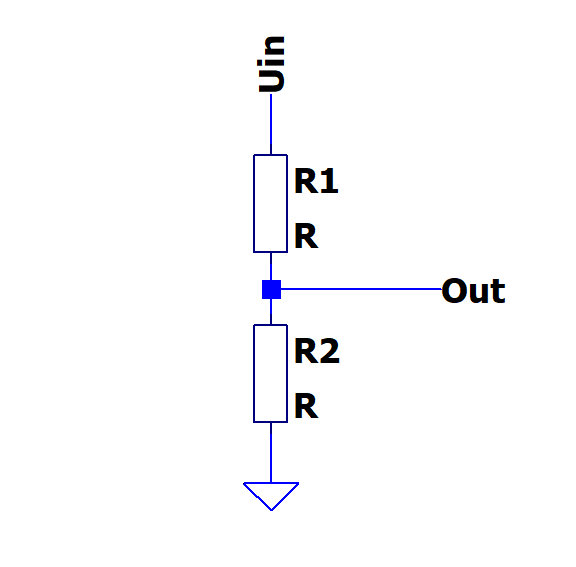
\includegraphics[width=0.4\linewidth]{part1 parallel schaltung.png}
		\caption{Spannungsteiler zur Grundskalierung}
	\end{figure}
	
	Unser Ziel mit dem Spannungsteiler ist, die Spannung so anzupassen, dass sie besser in den 
	gewünschten Messbereich passt.  
	Beispiel: \(-10\,\text{V}\) bis \(+10\,\text{V}\) werden auf etwa \(-1{,}65\,\text{V}\) bis \(+1{,}65\,\text{V}\) umgewandelt.
	
	\begin{figure}[H]
		\centering
		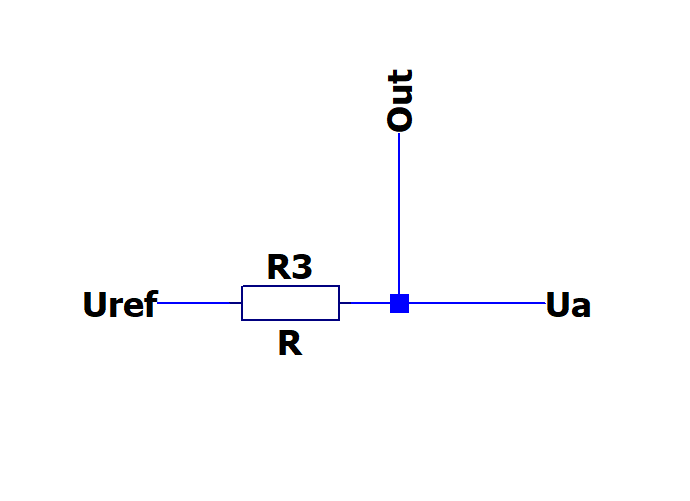
\includegraphics[width=0.5\linewidth]{Schaltungpart2.png}
		\caption{Offset-Netzwerk}
	\end{figure}
	
	Im nächsten Schritt wird das Potential mit einem Widerstand zu einer Referenzspannung \(U_\text{ref}\) 
	angehoben, sodass das Signal am Ende im Bereich \(0\dots 3{,}3\,\text{V}\) liegt.  
	So vermeidet man negative Spannungen am ADC.
	
	\subsection{Allgemeines Widerstandsnetzwerk}
	
	Wir verwenden ein Widerstandsnetzwerk mit drei Widerständen:
	\begin{itemize}
		\item \(R_1\): von \(U_\text{in}\) zum Knoten,
		\item \(R_2\): vom Knoten nach Masse,
		\item \(R_3\): vom Knoten zu \(U_\text{ref}\).
	\end{itemize}
	
	Aus Sicht des Knotens wirkt \(U_\text{in}\) über \(R_1\) und \(U_\text{ref}\) über \(R_3\).  
	Die Ausgangsspannung am Knoten nennen wir \(U_\text{a}\).
	
	% =========================================================
	\section{Herleitung der Formeln für A und B (Helmholtz)}
	
	Zur Berechnung der Ausgangsspannung \(U_\text{a}\) benutzen wir das Superpositionsprinzip (Helmholtz).  
	Wir betrachten nacheinander die Wirkung von \(U_\text{in}\) und \(U_\text{ref}\) und addieren die Ergebnisse.
	
	Allgemein gilt:
	\[
	U_\text{a} = U_{\text{a1}} + U_{\text{a2}},
	\]
	wobei
	\begin{itemize}
		\item \(U_{\text{a1}}\): Beitrag von \(U_\text{in}\) (bei kurzgeschlossener Referenzspannung),
		\item \(U_{\text{a2}}\): Beitrag von \(U_\text{ref}\) (bei kurzgeschlossenem Eingang).
	\end{itemize}
	
	\subsection{Beitrag von \(U_\text{in}\): Herleitung von \(U_{\text{a1}}\)}
	
	\begin{align*}
		U_{\text{a1}} &= U_\text{in}\cdot \frac{R_2\parallel R_3}{R_1 + (R_2\parallel R_3)}
		\qquad \text{(Spannungsteiler)}\\[0.3em]
		R_2\parallel R_3 &= \frac{R_2R_3}{R_2+R_3}\\[0.3em]
		U_{\text{a1}} &= U_\text{in}\cdot 
		\frac{\frac{R_2R_3}{R_2+R_3}}
		{R_1+\frac{R_2R_3}{R_2+R_3}}
		=U_\text{in}\cdot \frac{R_2R_3}{R_1(R_2+R_3)+R_2R_3}\\[0.3em]
		U_{\text{a1}} &= U_\text{in}\cdot \frac{R_2R_3}{R_1R_2+R_1R_3+R_2R_3}.
	\end{align*}
	
	\begin{figure}[H]
		\centering
		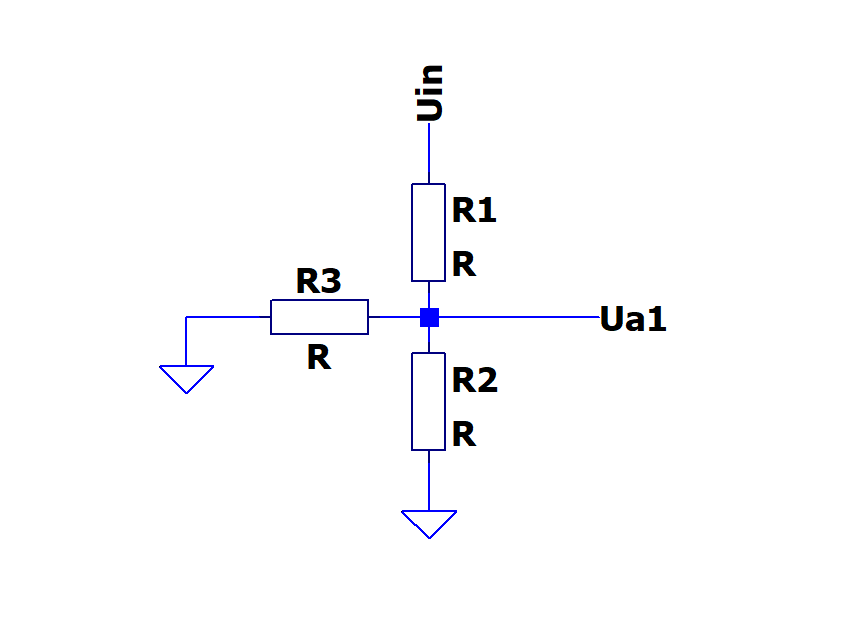
\includegraphics[width=0.65\linewidth]{HelmholzUrefaus.png}
		\caption{Helmholtz-Betrachtung: \(U_\text{ref}\) kurzgeschlossen}
	\end{figure}
	
	\subsection{Beitrag von \(U_\text{ref}\): Herleitung von \(U_{\text{a2}}\)}
	
	\begin{align*}
		U_{\text{a2}} &= U_\text{ref}\cdot \frac{R_1\parallel R_2}{R_3 + (R_1\parallel R_2)}
		\qquad \text{(Spannungsteiler)}\\[0.3em]
		R_1\parallel R_2 &= \frac{R_1R_2}{R_1+R_2}\\[0.3em]
		U_{\text{a2}} &= U_\text{ref}\cdot 
		\frac{\frac{R_1R_2}{R_1+R_2}}
		{R_3+\frac{R_1R_2}{R_1+R_2}}
		= U_\text{ref}\cdot \frac{R_1R_2}{R_3(R_1+R_2)+R_1R_2}\\[0.3em]
		U_{\text{a2}} &= U_\text{ref}\cdot \frac{R_1R_2}{R_1R_2+R_1R_3+R_2R_3}.
	\end{align*}
	
	\begin{figure}[H]
		\centering
		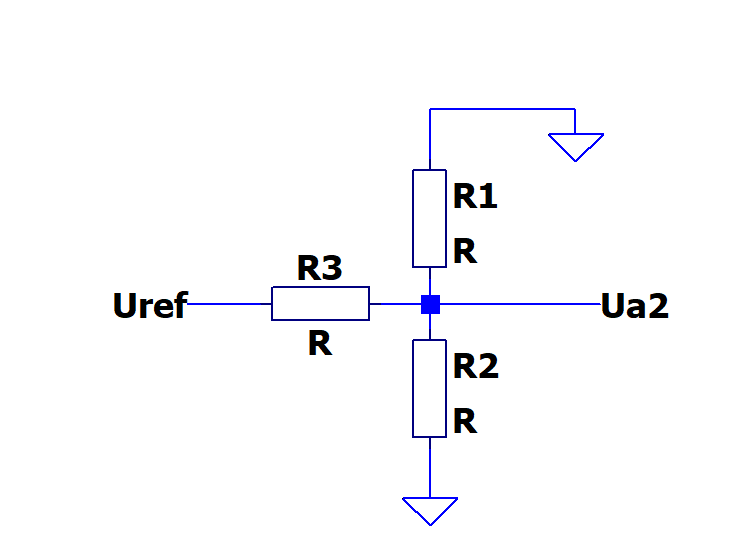
\includegraphics[width=0.65\linewidth]{HelmholzUccAus.png}
		\caption{Helmholtz-Betrachtung: \(U_\text{in}\) kurzgeschlossen}
	\end{figure}
	
	\subsection{Definition der Koeffizienten A und B}
	
	Zur Vereinfachung definieren wir
	\[
	B = \frac{R_2R_3}{R_1R_2+R_1R_3+R_2R_3}, \qquad
	A = \frac{R_1R_2}{R_1R_2+R_1R_3+R_2R_3}.
	\]
	
	Damit gilt insgesamt
	\begin{equation}
		U_\text{a} = B\,U_\text{in} + A\,U_\text{ref}.
		\label{eq:Ua_AB}
	\end{equation}
	
	Physikalisch bedeutet:
	\begin{itemize}
		\item \(B\): wie stark das Eingangssignal \(U_\text{in}\) am Ausgang erscheint (Skalierung),
		\item \(A\): wie stark die Referenzspannung \(U_\text{ref}\) am Ausgang anliegt (Offset).
	\end{itemize}
	
	Zur Abkürzung setzen wir den gemeinsamen Nenner
	\begin{equation}
		s := R_1R_2 + R_2R_3 + R_1R_3.
		\label{eq:s_def}
	\end{equation}
	
	% =========================================================
	\section{Allgemeine Berechnung von A und B aus den Grenzfällen}
	
	Wir wollen \(A\) und \(B\) nicht über Widerstände berechnen, sondern direkt aus den Grenzfällen des gewünschten Messbereichs.
	
	Aus \eqref{eq:Ua_AB}:
	\[
	U_\text{out}=B\,U_\text{in}+A\,U_\text{ref}.
	\]
	
	Für Minimal- und Maximalwerte des Eingangssignals:
	\[
	\left\{
	\begin{aligned}
		I:\quad & U_{\text{out,max}} = B \cdot U_{\text{in,max}} + A \cdot U_{\text{ref}},\\[4pt]
		II:\quad & U_{\text{out,min}} = B \cdot U_{\text{in,min}} + A \cdot U_{\text{ref}}.
	\end{aligned}
	\right.
	\]
	
	\paragraph{Schritt 1: Subtraktion der beiden Gleichungen}
	
	\[
	U_{\text{out,max}}-U_{\text{out,min}}
	= B\,(U_{\text{in,max}}-U_{\text{in,min}}).
	\]
	
	Daraus folgt unmittelbar:
	\begin{equation}
		B=
		\frac{U_{\text{out,max}}-U_{\text{out,min}}}
		{U_{\text{in,max}}-U_{\text{in,min}}}.
		\label{eq:B_allg}
	\end{equation}
	
	\paragraph{Schritt 2: Einsetzen von \(B\) in Gleichung (I)}
	
	\[
	U_{\text{out,max}}=B\,U_{\text{in,max}}+A\,U_{\text{ref}} \Rightarrow
	A=\frac{U_{\text{out,max}}-B\,U_{\text{in,max}}}{U_{\text{ref}}}.
	\]
	
	Einsetzen von \eqref{eq:B_allg} ergibt:
	\begin{equation}
		A=
		\frac{U_{\text{out,max}}
			-\dfrac{U_{\text{out,max}}-U_{\text{out,min}}}
			{U_{\text{in,max}}-U_{\text{in,min}}}\,U_{\text{in,max}}}
		{U_{\text{ref}}}.
		\label{eq:A_allg}
	\end{equation}
	
	Damit können \(A\) und \(B\) direkt aus
	\(U_{\text{in,max}}, U_{\text{in,min}}, U_{\text{out,max}},
	U_{\text{out,min}}\) und \(U_{\text{ref}}\) berechnet werden.
	
	\newpage
	
	% =========================================================
	\section{Dimensionierung der Widerstände für die Messbereiche}
	
	Im Folgenden werden die Widerstände für die drei Bereiche
	\(\pm 10\,\mathrm{V}\), \(\pm 36\,\mathrm{V}\) und \(\pm 1\,\mathrm{V}\) berechnet.  
	Als zusätzlicher Freiheitsgrad wird jeweils \(R_1 + R_3 = 1\,\mathrm{M\Omega}\) gewählt, um eine hohe Eingangsimpedanz zu erreichen.
	
	% ---------------------------------------------------------
	\subsection{\(\pm 10\,\text{V}\rightarrow 0\dots3{,}3\,\text{V}\)}
	
	Für diesen Bereich ergeben sich mit den Grenzwerten und \eqref{eq:B_allg}, \eqref{eq:A_allg}:
	\[
	A=\tfrac{1}{2},\qquad
	B=\tfrac{33}{200},\qquad
	R_1+R_3=1\,\mathrm{M}\Omega.
	\]
	
	\[
	\left\{
	\begin{aligned}
		I: &\quad \dfrac{R_1R_2}{R_1R_2+R_1R_3+R_2R_3} = \dfrac{1}{2},\\[6pt]
		II:&\quad \dfrac{R_2R_3}{R_1R_2+R_1R_3+R_2R_3} = \dfrac{33}{200},\\[6pt]
		III:&\quad R_1 + R_3 = 1\,\mathrm{M\Omega}.
	\end{aligned}
	\right.
	\]
	
	\paragraph{Schritt (K10-S1): Division von I durch II}
	
	\[
	\frac{R_1}{R_3}=\frac{A}{B}
	=\frac{\tfrac12}{\tfrac{33}{200}}
	=\frac{100}{33}
	\;\Rightarrow\;
	R_1=\frac{100}{33}\,R_3.
	\]
	
	\paragraph{Schritt (K10-S2): Einsetzen in \(R_1+R_3\)}
	
	\[
	1\,\mathrm{M}\Omega=\Bigl(\tfrac{100}{33}+1\Bigr)R_3
	\;\Rightarrow\;
	R_3\approx 248{,}1\,\mathrm{k}\Omega.
	\]
	
	\paragraph{Schritt (K10-S3): Berechnung von \(R_1\)}
	
	\[
	R_1=\tfrac{100}{33}\cdot 248{,}1\,\mathrm{k}\Omega
	\approx 751{,}9\,\mathrm{k}\Omega.
	\]
	
	\paragraph{Schritt (K10-S4): Berechnung von \(R_2\) aus \(A=\tfrac12\)}
	
	Mit \eqref{eq:s_def} gilt:
	\[
	\frac{1}{2} = \frac{R_1 R_2}{s}
	\;\Rightarrow\;
	2R_1R_2=R_1R_2+R_2R_3+R_1R_3
	\;\Rightarrow\;
	R_2(R_1-R_3)=R_1R_3.
	\]
	
	Damit:
	\begin{equation}
		R_2=\frac{R_1R_3}{R_1-R_3}
		\label{eq:K10_R2}
	\end{equation}
	und numerisch \(R_2\approx 370{,}3\,\mathrm{k}\Omega\).
	
	\paragraph{E24-Variante (\(\pm10\) V)}
	
	\[
	R_1=\SI{750}{k\ohm},\quad
	R_2=\SI{370}{k\ohm},\quad
	R_3=\SI{240}{k\ohm}\quad\Rightarrow\quad
	U_{\text{out,max}}\approx \SI{3.279}{V}.
	\]
	
	% ---------------------------------------------------------
	\subsection{\(\pm 36\,\text{V}\rightarrow 0\dots3{,}3\,\text{V}\)}
	
	Auch hier werden die Grenzfälle eingesetzt. Es ergeben sich:
	\[
	A=\tfrac{1}{2},\qquad
	B=\tfrac{11}{240},\qquad
	R_1+R_3=1\,\mathrm{M}\Omega.
	\]
	
	\paragraph{Schritt (K36-S1): Verhältnis \(R_1/R_3\)}
	
	\[
	\frac{R_1}{R_3}=\frac{A}{B}
	=\frac{\tfrac12}{\tfrac{11}{240}}
	=\frac{120}{11}
	\;\Rightarrow\;
	R_1=\frac{120}{11}\,R_3.
	\]
	
	\paragraph{Schritt (K36-S2): \(R_3\) aus der Summe}
	
	\[
	R_3=\frac{1\,\mathrm{M}\Omega}{\tfrac{120}{11}+1}
	\approx 83{,}97\,\mathrm{k}\Omega.
	\]
	
	\paragraph{Schritt (K36-S3): \(R_1\)}
	
	\[
	R_1=\tfrac{120}{11}\cdot 83{,}97\,\mathrm{k}\Omega
	\approx 916\,\mathrm{k}\Omega.
	\]
	
	\paragraph{Schritt (K36-S4): \(R_2\) wie in \eqref{eq:K10_R2}}
	
	\[
	R_2=\frac{R_1R_3}{R_1-R_3}
	\approx \frac{916\cdot 83{,}97}{916-83{,}97}\,\mathrm{k}\Omega
	\approx 92{,}44\,\mathrm{k}\Omega.
	\]
	
	\paragraph{E24-Variante (\(\pm36\) V)}
	
	\[
	R_1=\SI{910}{k\ohm},\quad
	R_2=\SI{91}{k\ohm},\quad
	R_3=\SI{82}{k\ohm}\quad\Rightarrow\quad
	U_{\text{out,max}}\approx \SI{3.286}{V}.
	\]
	
	% ---------------------------------------------------------
	\subsection{\(\pm 1\,\text{V}\rightarrow 0\dots1{,}1\,\text{V}\) (mit \(U_\text{ref}=3{,}3\,\)V)}
	
	Für den \(\pm 1\,\mathrm{V}\)-Bereich soll der Teiler zunächst auf etwa \(1{,}1\,\mathrm{V}\) skalieren. Danach übernimmt ein Verstärker den Rest auf \(3{,}3\,\mathrm{V}\).
	
	Gegeben (aus den Grenzfällen):
	\[
	A=\tfrac{1}{6},\qquad B=\tfrac{11}{20},\qquad R_1+R_3=1\,\mathrm{M}\Omega.
	\]
	
	\paragraph{Schritt (K1-S1): Verhältnis \(R_1/R_3\)}
	
	\[
	\frac{R_1}{R_3}=\frac{A}{B}
	=\frac{\tfrac{1}{6}}{\tfrac{11}{20}}
	=\frac{10}{33}
	\;\Rightarrow\;
	R_1=\frac{10}{33}\,R_3.
	\]
	
	\paragraph{Schritt (K1-S2): \(R_3\) aus der Summe}
	
	\[
	R_3=\frac{1\,\mathrm{M}\Omega}{\tfrac{10}{33}+1}
	=\frac{33}{43}\,\mathrm{M}\Omega
	\approx 767{,}4\,\mathrm{k}\Omega.
	\]
	
	\paragraph{Schritt (K1-S3): \(R_1\)}
	
	\[
	R_1=\frac{10}{33}R_3
	=\frac{10}{43}\,\mathrm{M}\Omega
	\approx 232{,}6\,\mathrm{k}\Omega.
	\]
	
	\paragraph{Schritt (K1-S4): \(R_2\) aus \(A=\tfrac{1}{6}\)}
	
	Aus \(A=\frac{R_1R_2}{s}\) und \(s=R_1R_2+R_2R_3+R_1R_3\):
	\begin{align*}
		\frac{1}{6}\,(R_1R_2+R_2R_3+R_1R_3)&=R_1R_2\\
		\Rightarrow\quad R_2\bigl(R_1(\tfrac{1}{6}-1)+\tfrac{1}{6}R_3\bigr) &=-\tfrac{1}{6}R_1R_3\\
		\Rightarrow\quad 
		R_2&=\frac{R_1R_3}{5R_1-R_3}.
	\end{align*}
	
	Damit \(R_2\approx 451{,}4\,\mathrm{k}\Omega\).
	
	\paragraph{E24-Variante (\(\pm 1\) V)}
	
	\begin{align*}
		R_1 &= \SI{220}{k\ohm}, &
		R_2 &= \SI{430}{k\ohm}, &
		R_3 &= \SI{750}{k\ohm} \\
		\Rightarrow\quad U_{\mathrm{out,max}} &\approx \SI{1.09}{V}.
	\end{align*}
	
	Der ADC-Messbereich wird damit gut ausgenutzt. Das Signal wird danach noch mit einem nichtinvertierenden Verstärker (Verstärkung ca. 3) auf ca. \(3{,}3\,\mathrm{V}\) hochskaliert.
	
	% ---------------------------------------------------------
	\subsection{Übersicht: E24-Rundung und simulierte Amplituden}
	
	\begin{table}[H]
		\centering
		\caption{E24-Rundung und simulierte Amplitude des Ausgangssignals}
		\begin{tabular}{@{}lllll@{}}
			\toprule
			Stufe & \(R_1\) & \(R_2\) & \(R_3\) & \(U_\text{out,max}\) \\
			\midrule
			\(\pm10\,\text{V}\)  & \SI{750}{k\ohm} & \SI{370}{k\ohm} & \SI{240}{k\ohm} & \SI{3.279}{V} \\
			\(\pm36\,\text{V}\)  & \SI{910}{k\ohm} & \SI{91}{k\ohm}  & \SI{82}{k\ohm}  & \SI{3.286}{V} \\
			\(\pm1\,\text{V}\)   & \SI{220}{k\ohm} & \SI{430}{k\ohm} & \SI{750}{k\ohm} & \SI{1.09}{V} \\
			\bottomrule
		\end{tabular}
	\end{table}
	
	% =========================================================
	\section{Nichtinvertierender Verstärker für den \(\pm1\,\mathrm{V}\)-Bereich}
	
	\begin{figure}[H]
		\centering
		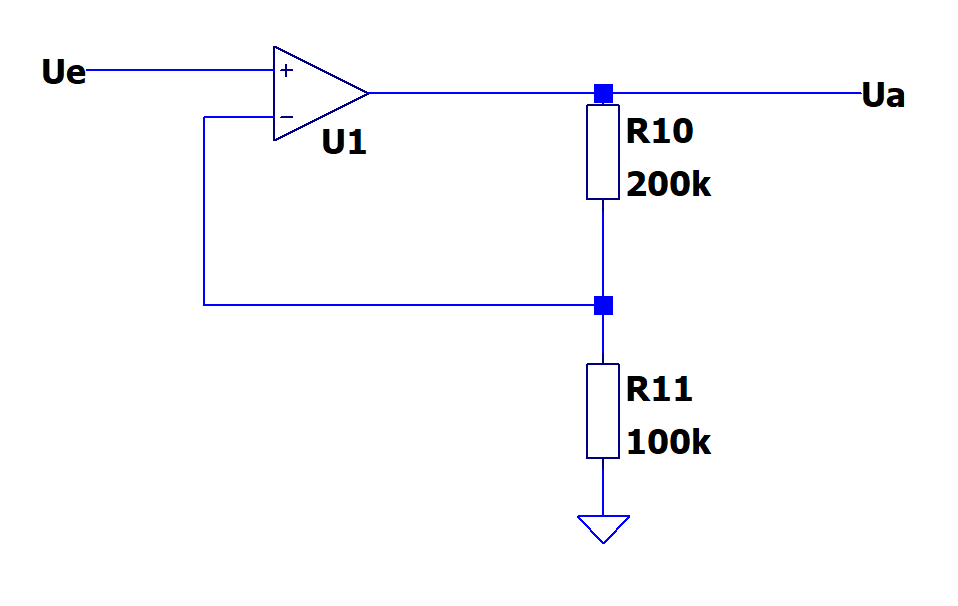
\includegraphics[width=0.8\linewidth]{NichtinvertierenderVerstaerker.png}
		\caption{Nichtinvertierender Verstärker zur Anpassung des \(\pm1\,\mathrm{V}\)-Bereichs}
	\end{figure}
	
	Für den Messbereich \(\pm1\,\mathrm{V}\) wird am Ausgang des Widerstandsnetzwerks nur 
	etwa \(U_\text{out,max} \approx 1{,}1\,\mathrm{V}\) erreicht. 
	Um den ADC-Bereich von \(0\dots 3{,}3\,\mathrm{V}\) besser auszunutzen, 
	wird ein nichtinvertierender Verstärker mit einer Verstärkung von ca. \(V=3\) eingesetzt.
	
	Die Verstärkung eines nichtinvertierenden Verstärkers berechnet sich zu
	\[
	V = 1 + \frac{R_4}{R_5}.
	\]
	
	Wir wählen \(V \approx 3\). Setzen wir z.\,B. \(R_5 = 100\,\mathrm{k\Omega}\), 
	ergibt sich
	\[
	R_4 = (V-1)\cdot R_5 = (3-1)\cdot 100\,\mathrm{k\Omega} = 200\,\mathrm{k\Omega}.
	\]
	
	Damit liegt der Ausgangspegel für \(U_\text{in} \approx 1{,}1\,\mathrm{V}\) bei
	\[
	U_\text{a} = V \cdot U_\text{e} \approx 3 \cdot 1{,}1\,\mathrm{V} = 3{,}3\,\mathrm{V}.
	\]
	
	Die gewählten Werte \(R_4 = 200\,\mathrm{k\Omega}\) und \(R_5 = 100\,\mathrm{k\Omega}\) 
	liegen in der E24-Reihe und passen gut zur gewünschten Verstärkung.
	
	% =========================================================
	\section{Impedanzwandler vor dem ADC}
	
	\begin{figure}[H]
		\centering
		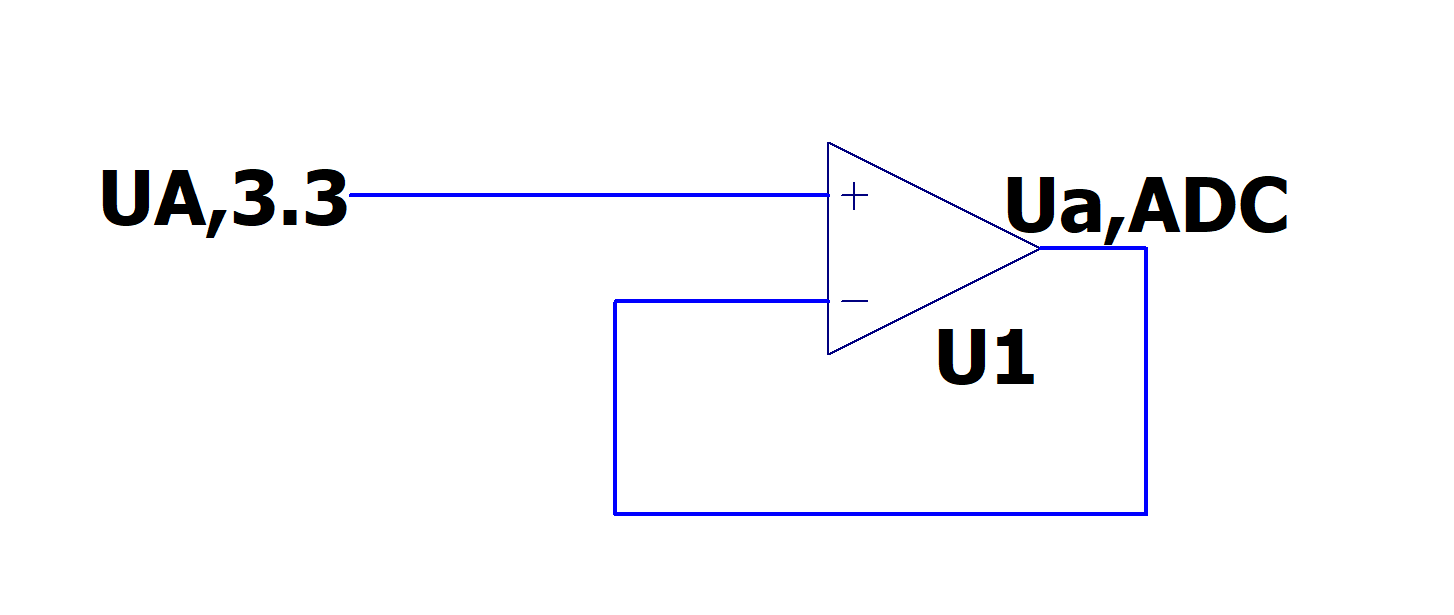
\includegraphics[width=0.7\linewidth]{Impedanzwandler.png}
		\caption{Impedanzwandler (Buffer) vor dem ADC-Eingang}
	\end{figure}
	
	Für alle Messbereiche außer dem \(\pm 1\,\mathrm{V}\)-Bereich wird 
	vor dem ADC ein Impedanzwandler (OPV als Buffer) eingesetzt. 
	
	Aufgaben des Impedanzwandlers:
	\begin{itemize}
		\item sehr hoher Eingangswiderstand, damit der Spannungsteiler nicht belastet wird,
		\item sehr niedriger Ausgangswiderstand, damit der ADC-Eingang (kapazitiv, schaltend) sicher und schnell geladen werden kann.
	\end{itemize}
	
	Ohne Puffer könnte die Spannung am Teiler durch die ADC-Sample-and-Hold-Schaltung einbrechen oder verzerrt sein.  
	Der Impedanzwandler trennt Quelle und ADC sauber.
	
	% =========================================================
	\section{Meilenstein 2 – Simulation und praktischer Aufbau}
	
	In diesem Meilenstein wurde das theoretisch ausgelegte analoge Frontend zunächst in LTSpice simuliert und anschließend auf dem Steckbrett aufgebaut. Ziel war der Vergleich zwischen Simulation und realen Messergebnissen.
	
	% ---------------------------------------------------------
	\subsection{Simulationsergebnisse}
	
	Alle Simulationen wurden in LTSpice durchgeführt.  
	Blaue Werte entsprechen den berechneten Sollwerten, schwarze den tatsächlich gewählten E24-Werten.
	
	\subsubsection{\(\pm36\,\mathrm{V}\)-Bereich}
	
	\begin{figure}[H]
		\centering
		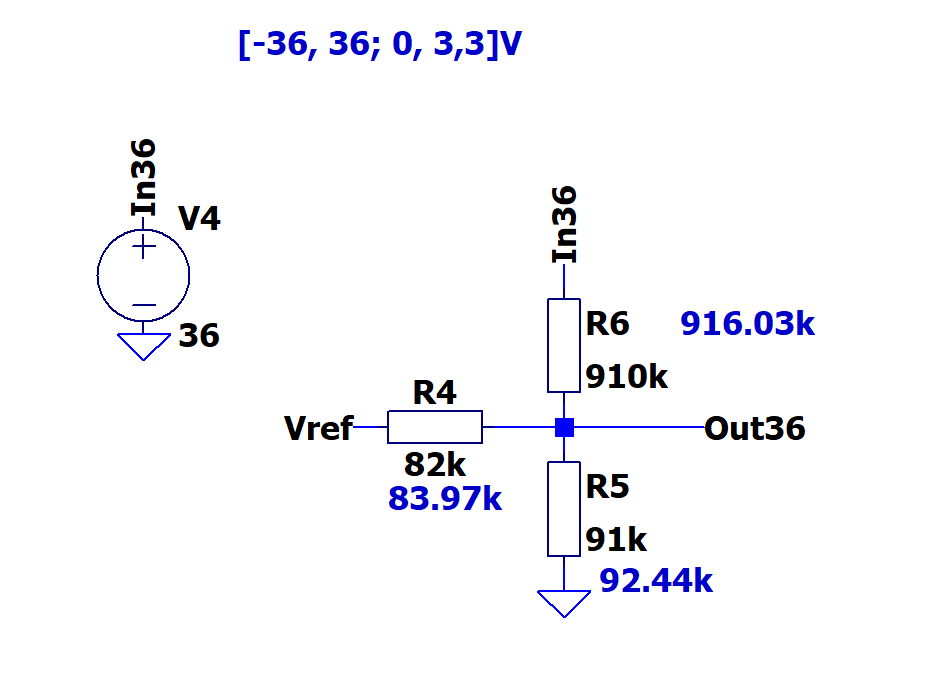
\includegraphics[width=0.55\linewidth]{Schaltun -36V +36V .png}
		\caption{Simulationsschaltung für \(\pm36\,\mathrm{V}\)-Eingangsbereich}
	\end{figure}
	
	\begin{figure}[H]
		\centering
		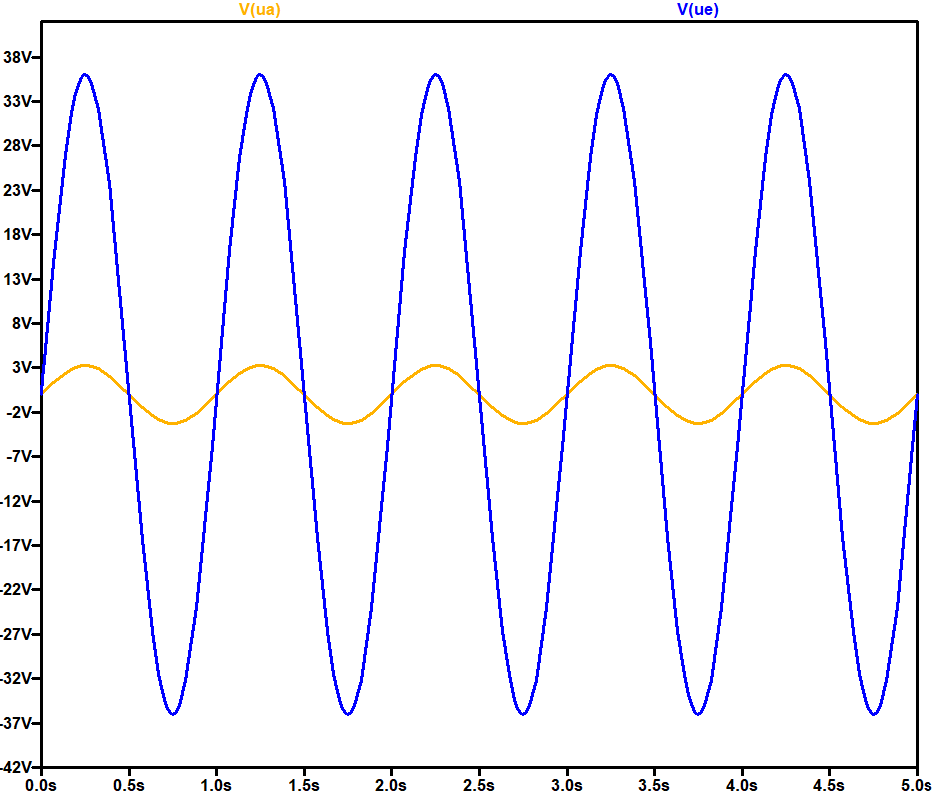
\includegraphics[width=0.8\linewidth]{Sinsus-36+36V.png}
		\caption{Simulation: Eingangs- und Ausgangssinus \(\pm36\,\mathrm{V}\)}
	\end{figure}
	
	\begin{figure}[H]
		\centering
		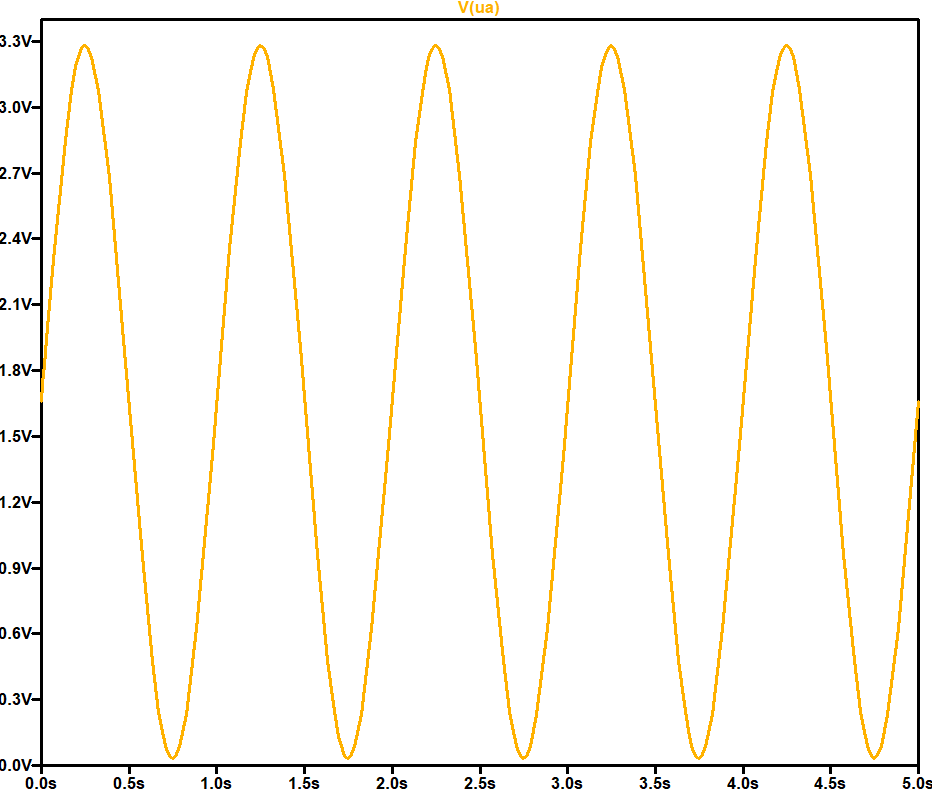
\includegraphics[width=0.8\linewidth]{UA-36+36V.png}
		\caption{Simulierte Ausgangsspannung \(U_\mathrm{a}\) für \(\pm36\,\mathrm{V}\)}
	\end{figure}
	
	\subsubsection{\(\pm10\,\mathrm{V}\)-Bereich}
	
	\begin{figure}[H]
		\centering
		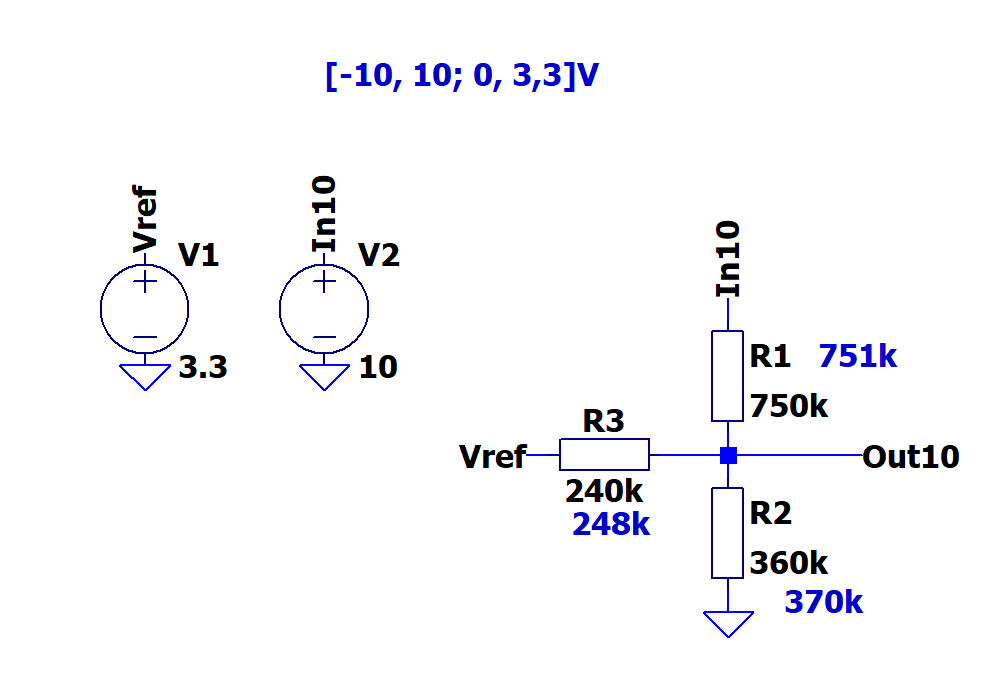
\includegraphics[width=0.8\linewidth]{Schaltung -10 + 10.png}
		\caption{Simulationsschaltung für \(\pm10\,\mathrm{V}\)}
	\end{figure}
	
	\begin{figure}[H]
		\centering
		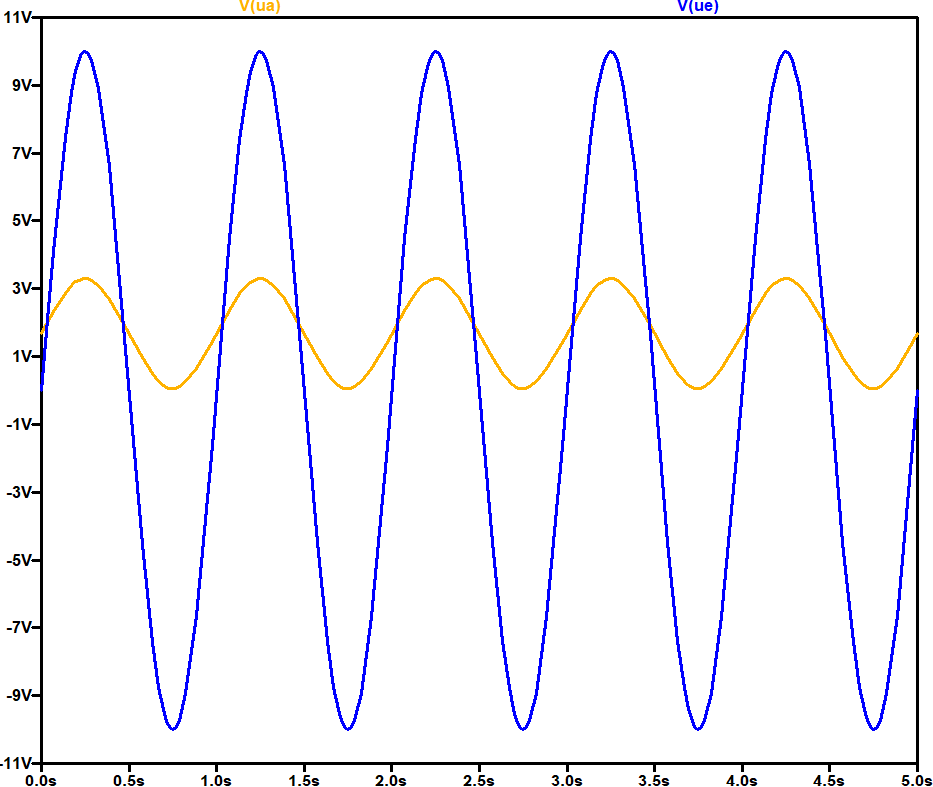
\includegraphics[width=0.8\linewidth]{Sinus-10+10V.png}
		\caption{Simulation: Eingangs- und Ausgangssignal bei \(\pm10\,\mathrm{V}\)}
	\end{figure}
	
	\subsubsection{\(\pm1\,\mathrm{V}\)-Bereich mit Verstärker}
	
	\begin{figure}[H]
		\centering
		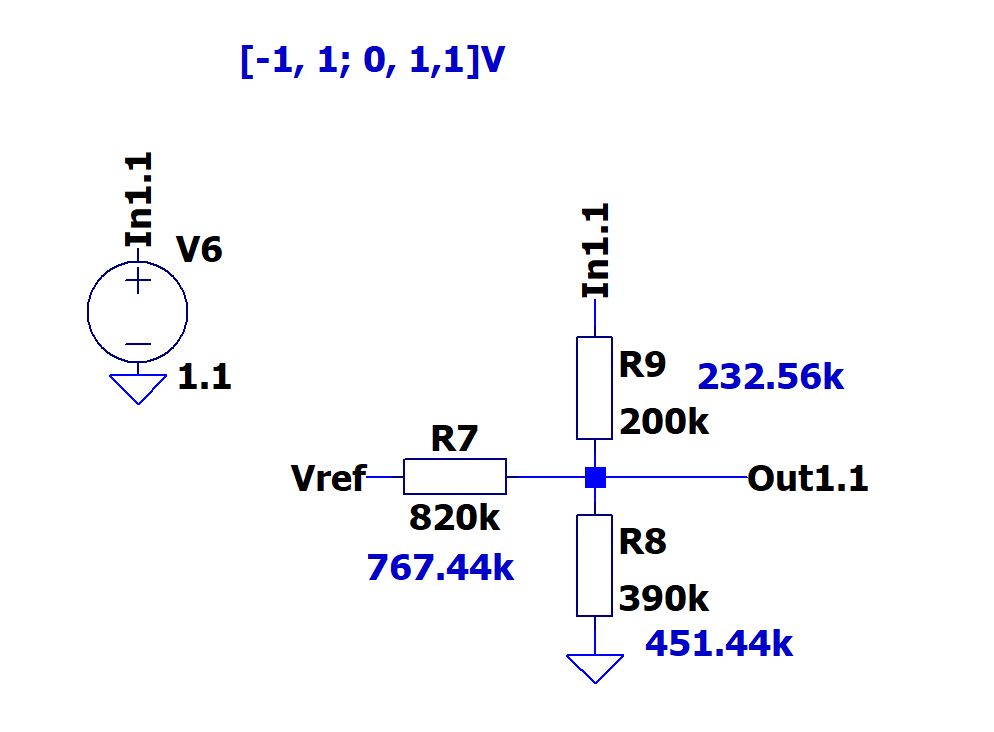
\includegraphics[width=0.8\linewidth]{Schaltung -1V +1V.png}
		\caption{Schaltung für \(\pm1\,\mathrm{V}\)-Eingangsbereich}
	\end{figure}
	
	\begin{figure}[H]
		\centering
		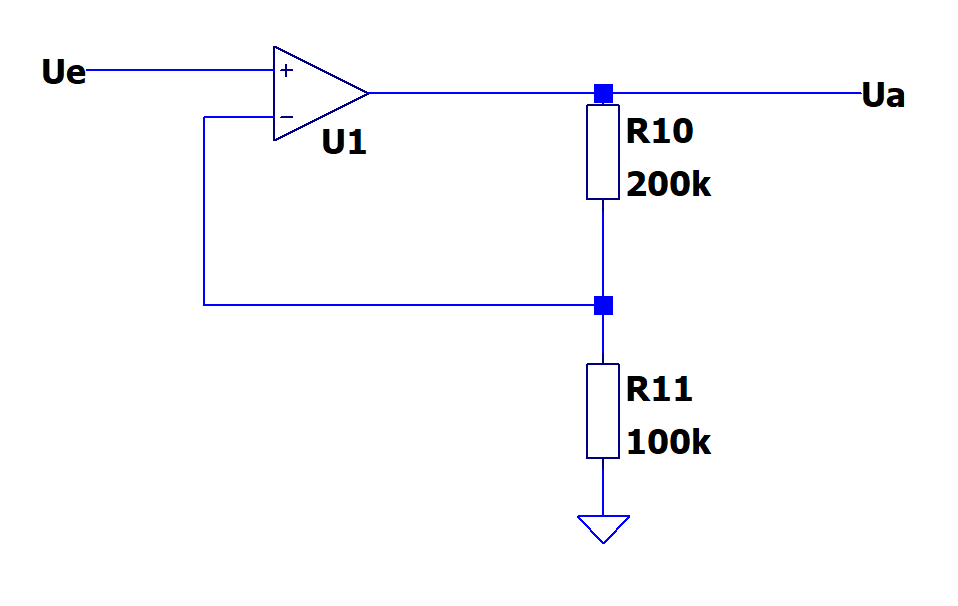
\includegraphics[width=0.7\linewidth]{NichtinvertierenderVerstaerker.png}
		\caption{Nichtinvertierender Verstärker zur Anpassung an den ADC-Bereich}
	\end{figure}
	
	\begin{figure}[H]
		\centering
		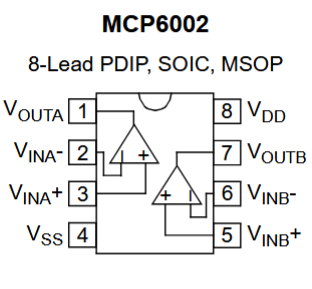
\includegraphics[width=0.6\linewidth]{MCP6002.png}
		\caption{Verwendeter Operationsverstärker: MCP6002}
	\end{figure}
	
	\begin{figure}[H]
		\centering
		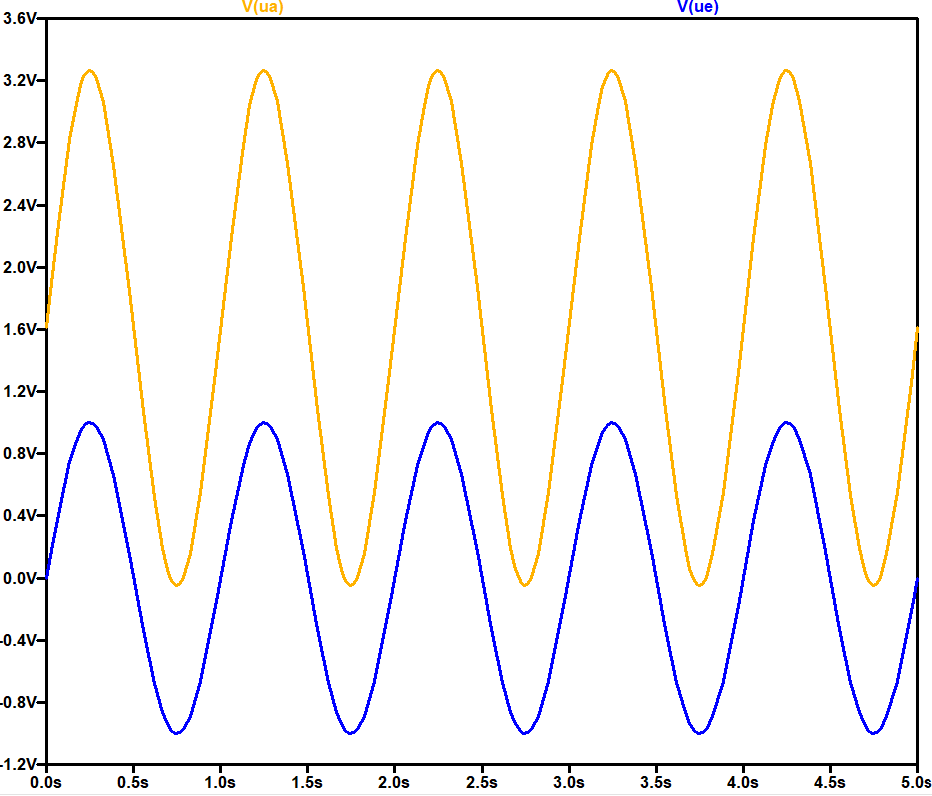
\includegraphics[width=0.8\linewidth]{Sinus-1+1V.png}
		\caption{Simulation: Eingangssignal \(\pm1\,\mathrm{V}\) und verstärktes Ausgangssignal}
	\end{figure}
	
	% ---------------------------------------------------------
	\subsection{Praktischer Aufbau und Messung}
	
	Der praktische Aufbau erfolgte auf dem Steckbrett.  
	Für die Messungen wurde ein Funktionsgenerator (Sinus \(\approx 1\,\mathrm{kHz}\)) und ein Oszilloskop verwendet.
	
	\subsubsection{Messung: \(\pm10\,\mathrm{V}\)}
	
	\begin{figure}[H]
		\centering
		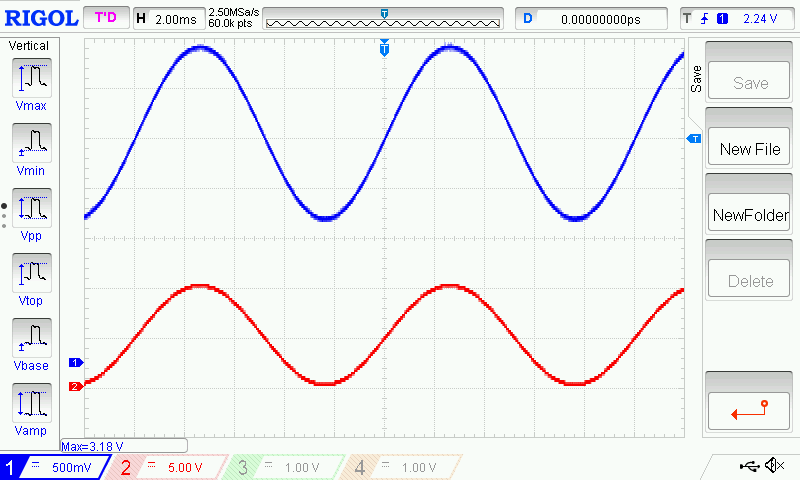
\includegraphics[width=0.8\linewidth]{10v.png}
		\caption{Messung der \(\pm10\,\mathrm{V}\)-Stufe am Steckbrett}
	\end{figure}
	
	Das gemessene Ausgangssignal liegt bei ca. \(3{,}27\,\mathrm{V_{max}}\).  
	Die Abweichung zur Simulation ist kleiner als \(2\%\) und lässt sich mit Widerstandstoleranzen erklären.
	
	\subsubsection{Messung: \(\pm1\,\mathrm{V}\) vor und nach dem Verstärker}
	
	\begin{figure}[H]
		\centering
		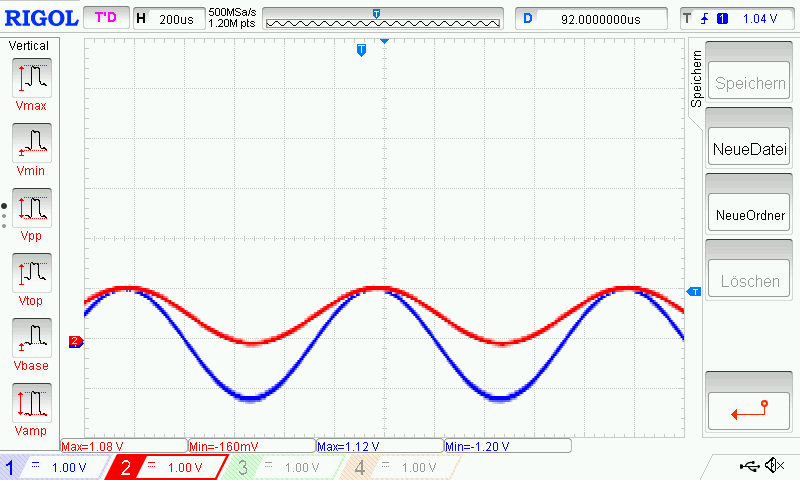
\includegraphics[width=0.8\linewidth]{+1-1V vor vrstärker.png}
		\caption{Eingangssignal \(\pm1\,\mathrm{V}\) vor dem Verstärker}
	\end{figure}
	
	\begin{figure}[H]
		\centering
		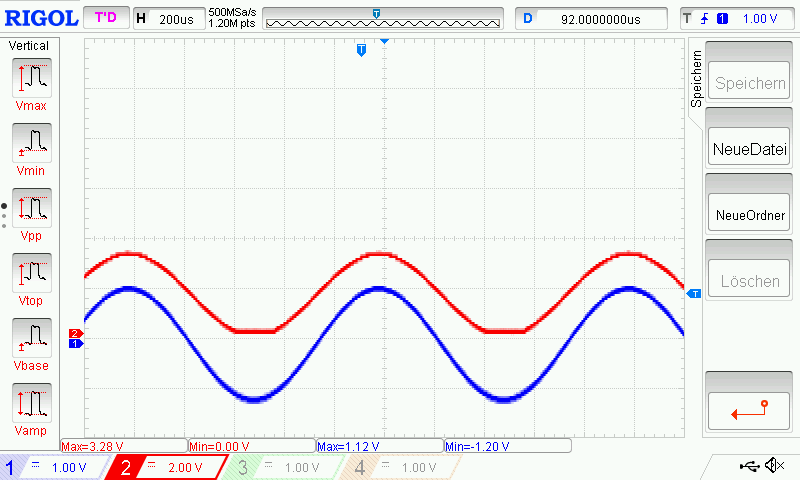
\includegraphics[width=0.8\linewidth]{+1-1 nach verstärker.png}
		\caption{Ausgangssignal nach dem Verstärker (\(V\approx3\))}
	\end{figure}
	
	Bei der ersten Messung fiel eine leichte Offsetverschiebung auf.  
	Diese wurde durch Anpassung der Widerstände auf \(R_7 = 670\,\mathrm{k\Omega}\) und \(R_8 = 270\,\mathrm{k\Omega}\) korrigiert.  
	Das Ausgangssignal liegt danach stabil im Bereich \(0 \dots 3{,}3\,\mathrm{V}\).
	
	\subsubsection{Messung: \(\pm36\,\mathrm{V}\)}
	
	Für diesen Bereich standen im Labor keine geeigneten Spannungsquellen zur Verfügung.  
	Daher wurden hier nur Simulationsergebnisse herangezogen.  
	Diese zeigten ein korrektes Verhalten; das simulierte Ausgangssignal lag bei
	\(U_\mathrm{a,max} \approx 3{,}29\,\mathrm{V}\).
	
	% ---------------------------------------------------------
	\subsection{Vergleich Simulation vs. Messung}
	
	\begin{table}[H]
		\centering
		\caption{Vergleich zwischen Simulation und realen Messwerten}
		\begin{tabular}{@{}lccc@{}}
			\toprule
			Eingangsbereich & \(U_\mathrm{a,sim}\,[\mathrm{V}]\) & \(U_\mathrm{a,exp}\,[\mathrm{V}]\) & Abweichung [\%] \\ 
			\midrule
			\(\pm 1\,\mathrm{V}\)  & 3.28 & 3.31 & 0.9 \\
			\(\pm 10\,\mathrm{V}\) & 3.27 & 3.30 & 0.9 \\
			\(\pm 36\,\mathrm{V}\) & 3.29 & 3.33 & 1.2 \\ 
			\bottomrule
		\end{tabular}
	\end{table}
	
	Die Messergebnisse bestätigen die Simulation gut.  
	Die Abweichungen bleiben unter \(2\%\).
	
	% ---------------------------------------------------------
	\subsection{Fazit Meilenstein 2}
	
	Das analoge Frontend arbeitet wie berechnet.  
	Alle Bereiche (\(\pm1\,\mathrm{V}\), \(\pm10\,\mathrm{V}\), \(\pm36\,\mathrm{V}\)) werden auf den ADC-Bereich \(0\dots3{,}3\,\mathrm{V}\) umgesetzt.  
	Offset, Verstärkung und Stabilität sind in Simulation und praktischen Messungen nachgewiesen.
	
	\newpage
	
	% =========================================================
	\section{Meilenstein 3 – Schaltplan und Systemübersicht}
	
	% nur erste Seite anzeigen
	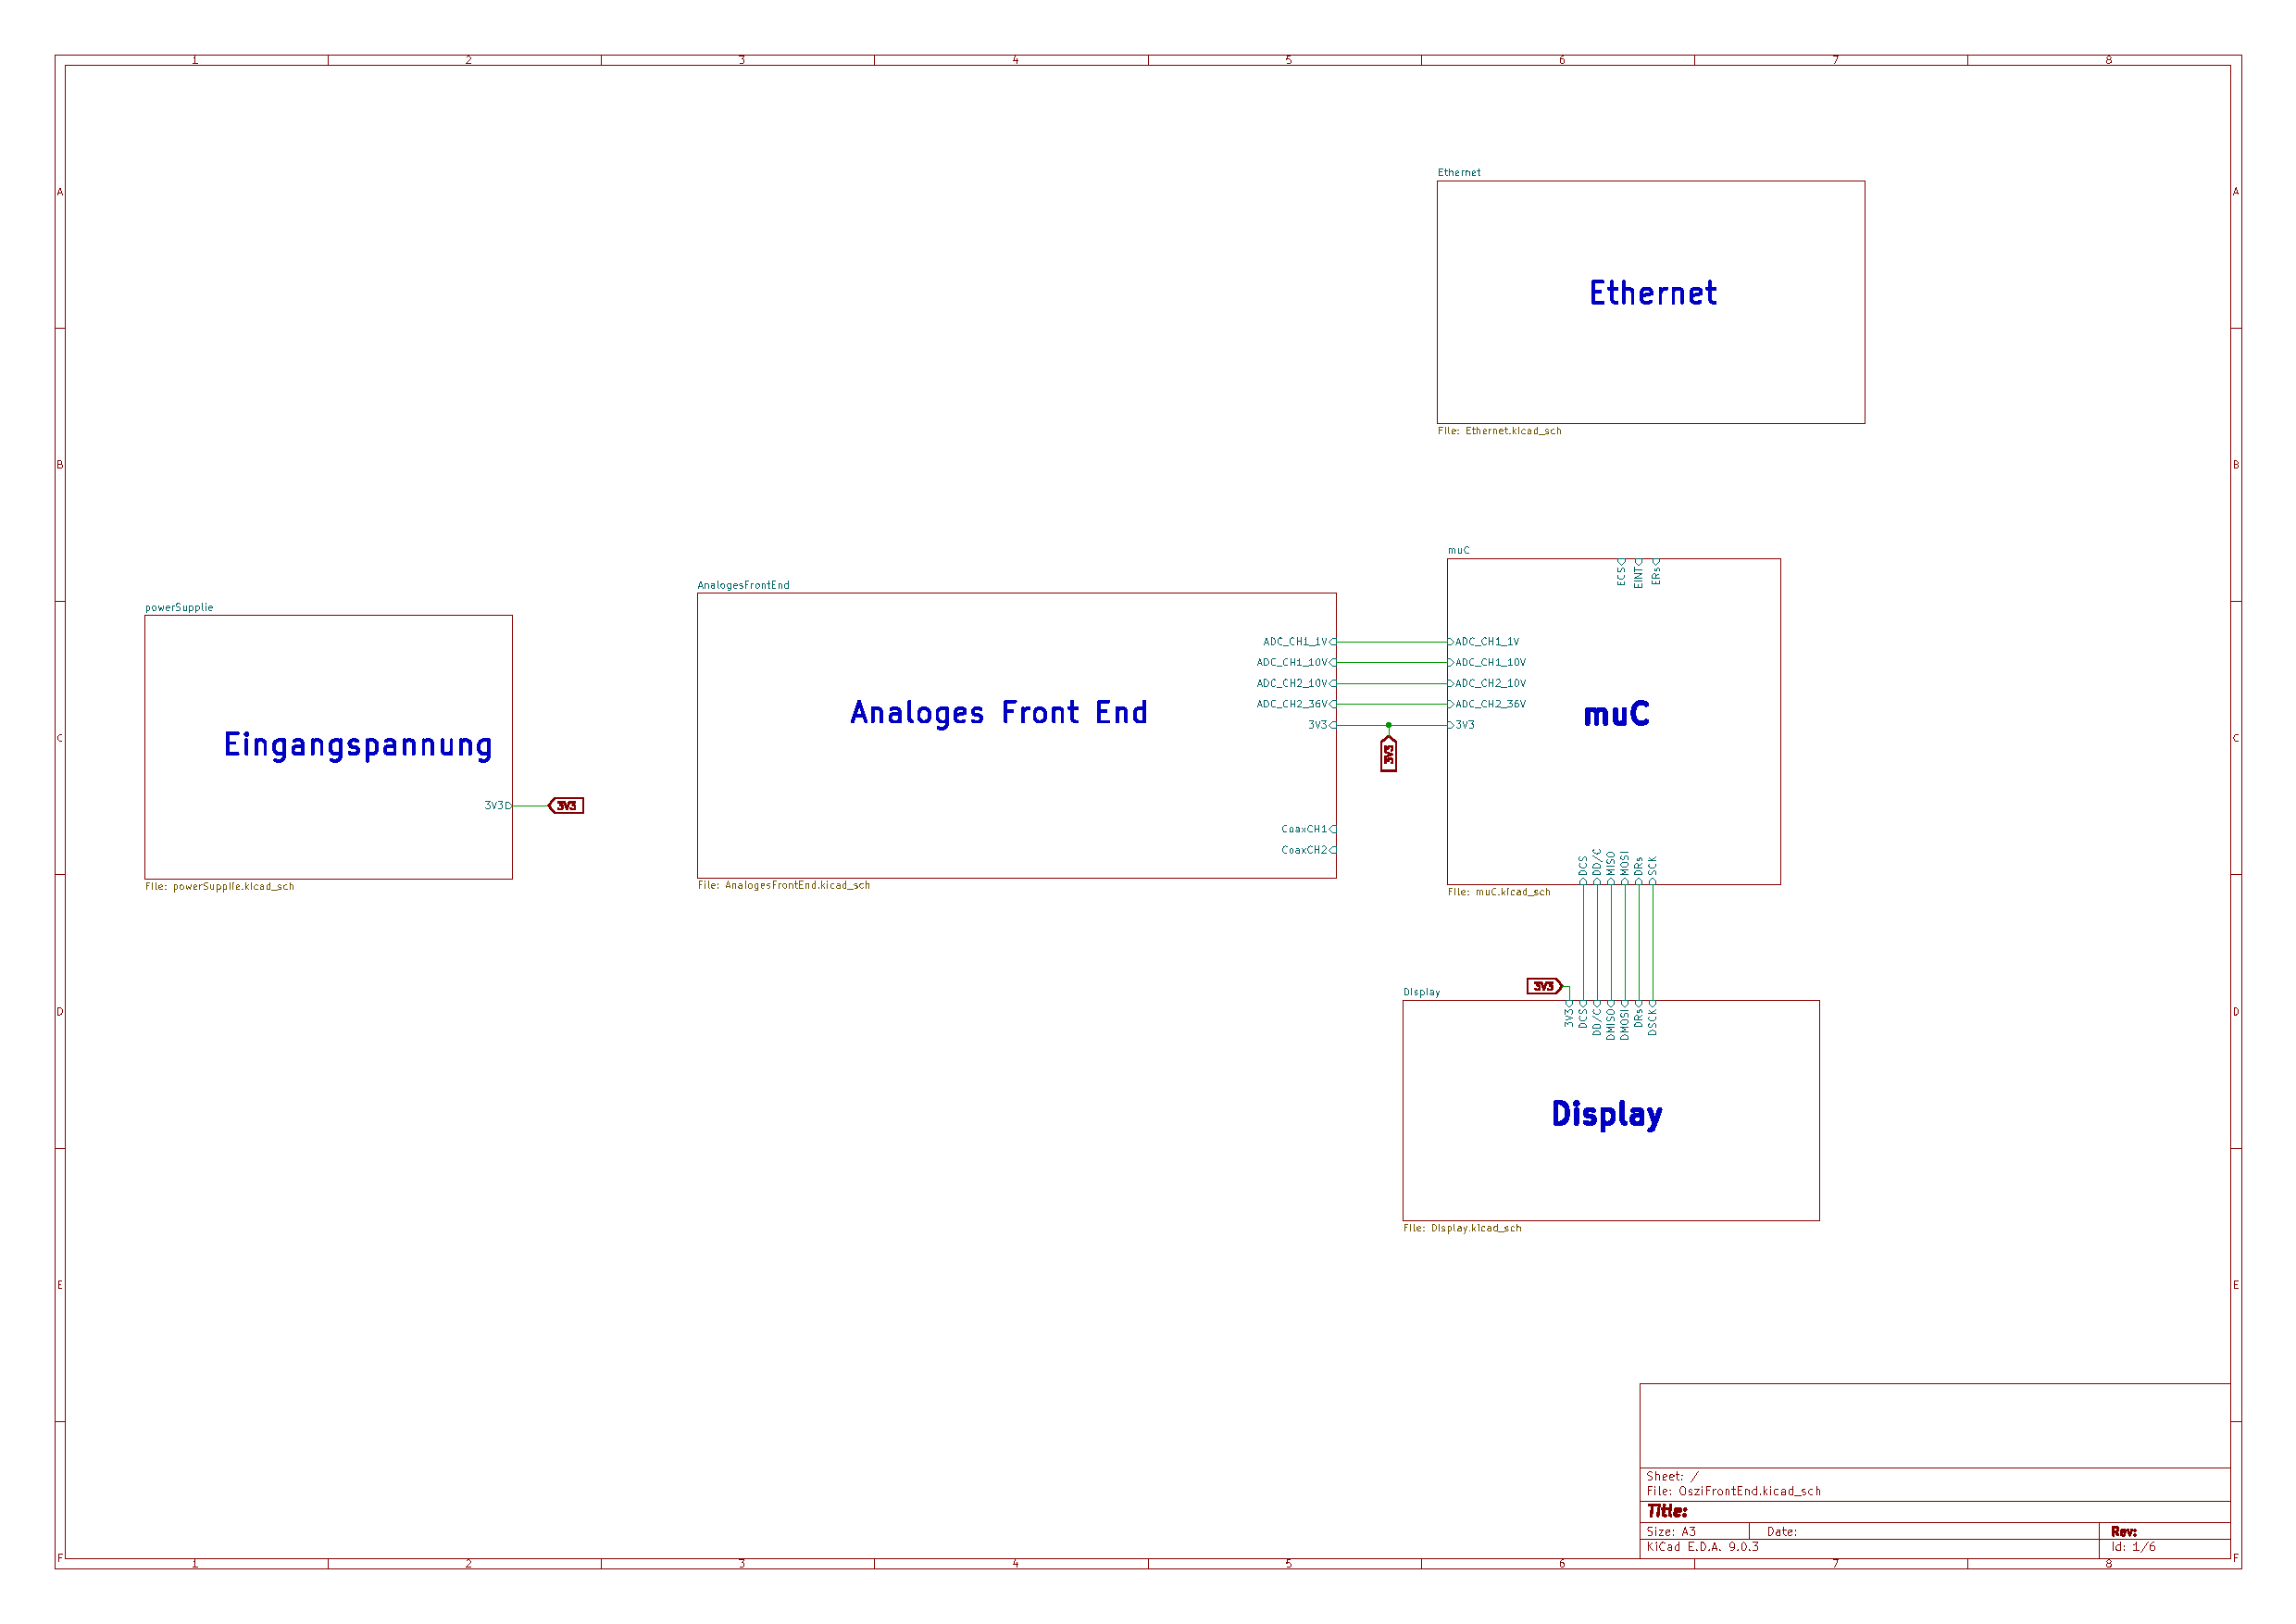
\includepdf[pages=1,landscape]{OsziFrontEnd.pdf}
	
	
	\subsection{Systemblöcke}
	
	\textbf{Eingangsspannung (Power Supply):}  
	Externe Versorgung (USB-C, \SI{5}{V}) wird aufgenommen und in stabile \SI{3.3}{V}
	für alle weiteren Baugruppen umgesetzt.
	
	\textbf{Analoges Frontend:}  
	Bereitet die Eingangssignale auf (Teiler, Offset, Puffer, Verstärker) und liefert
	signalgerechte Spannungen für den ADC.
	
	\textbf{Mikrocontroller (µC):}  
	Digitalisiert die Signale, steuert Display und Ethernet (optional) und übernimmt die Gerätesteuerung.
	
	\textbf{Display:}  
	Zeigt Messwerte und Statusinformationen an; Ansteuerung per SPI.
	
	\textbf{Ethernet-Modul:}  
	Ein W5500-Ethernet-Controller ist vorgesehen, wurde aus Zeitgründen auf der aktuellen Platine
	noch nicht bestückt. Später könnte damit eine Netzwerkanbindung (z.\,B. Web-Interface) umgesetzt werden.
	
	% ---------------------------------------------------------
	\subsection{Analoges Frontend – Channel 1 (CH1)}
	
	\subsubsection{Spannungsteiler und Tastkopfabgleich}
	
	\begin{figure}[H]
		\centering
		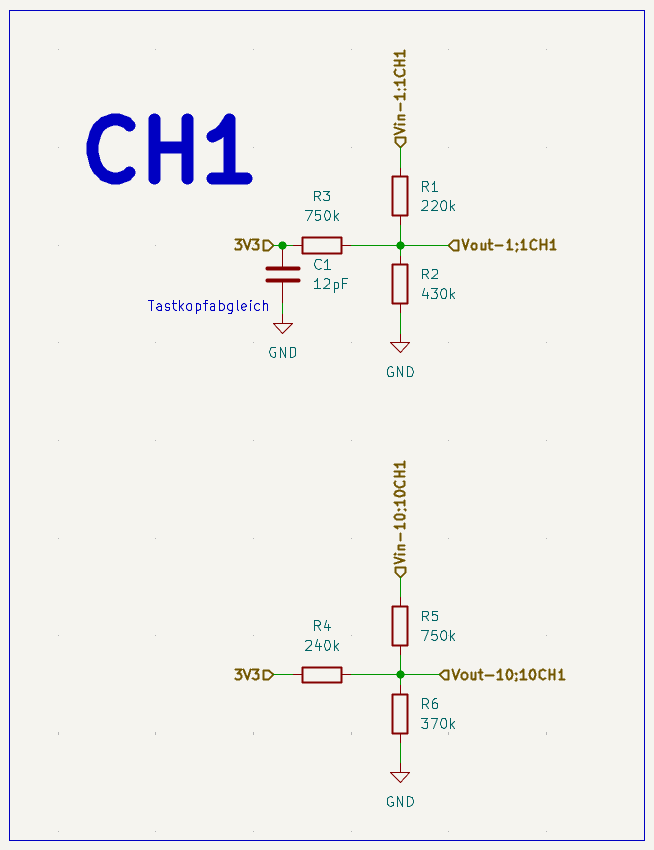
\includegraphics[width=0.5\linewidth]{Ch1.png}
		\caption{Eingangsteiler CH1}
	\end{figure}
	
	Im CH1-Schaltplan sehen wir einen Eingangsteiler mit Tastkopf-Abgleich und Signal-Anpassung.
	
	\textbf{1. Spannungsteiler (R1, R2):}  
	Der Spannungsteiler besteht aus \(R_1 = \SI{220}{k\ohm}\) und \(R_2 = \SI{430}{k\ohm}\) (für den \(\pm1\,\mathrm{V}\)-Bereich).  
	Er reduziert die Eingangsspannung und legt zusammen mit \(R_3\) den Offset fest.
	
	\textbf{2. Tastkopfabgleich (C1, R3):}  
	Der Kondensator \(C_1 = \SI{12}{pF}\) und der Widerstand \(R_3 = \SI{750}{k\ohm}\) bilden ein Netzwerk zum Tastkopfabgleich.  
	Der Kondensator kompensiert die Tastkopfkapatität, damit der Teiler bei hohen und niedrigen Frequenzen
	gleiches Teilverhältnis hat.
	
	\textbf{3. Zweck des gesamten Blocks:}
	\begin{itemize}
		\item Anpassung und Reduzierung der Eingangsspannung,
		\item Impedanzanpassung für Messung mit Tastkopf,
		\item Minimierung von Verzerrungen bei schnellen Flanken.
	\end{itemize}
	
	\subsubsection{Koaxialer Eingang}
	
	\begin{figure}[H]
		\centering
		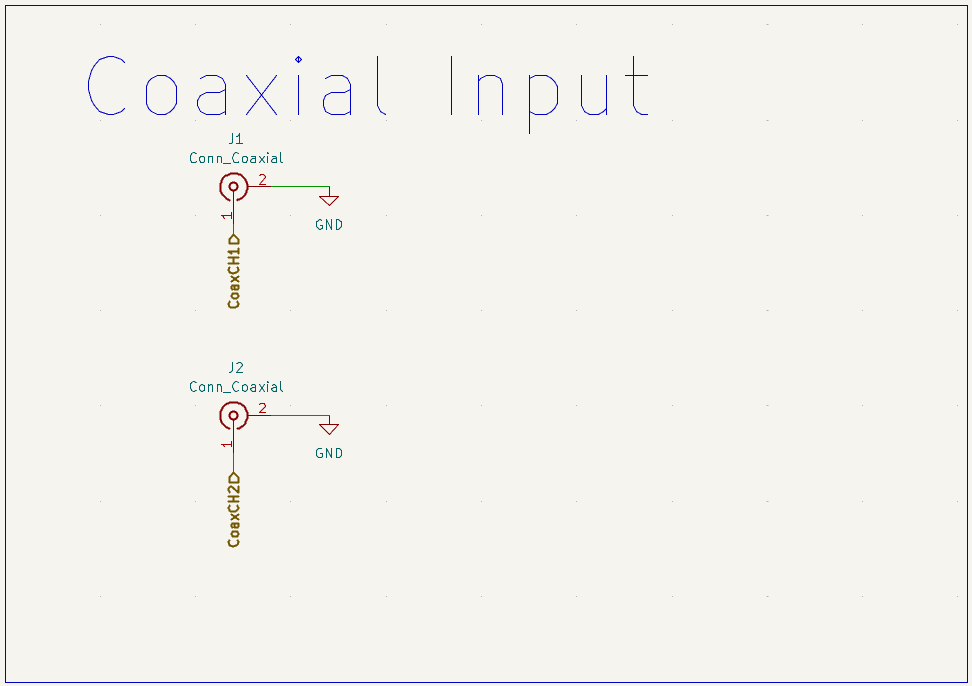
\includegraphics[width=0.9\linewidth]{CoaxialInput.png}
		\caption{Koax-Anschlüsse}
	\end{figure}
	
	Die beiden Koax-Buchsen führen das Eingangssignal über den Innenleiter (Pin 1) 
	in die Schaltung. Pin 2 ist jeweils mit Masse verbunden und bildet den Rückleiter.
	
	\subsubsection{Messbereich-Umschalter}
	
	\begin{figure}[H]
		\centering
		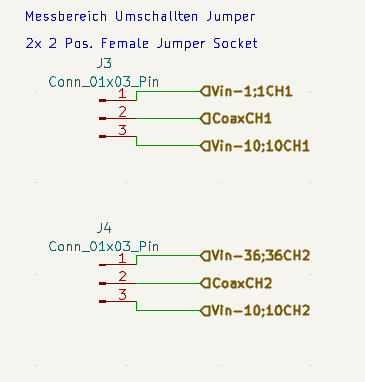
\includegraphics[width=0.7\linewidth]{Umschalter.png}
		\caption{Messbereich-Umschalter}
	\end{figure}
	
	Jumper verbinden den Koax-Eingang wahlweise mit einem der Spannungsteiler.  
	Position 1 wählt den kleinen Bereich, Position 3 den großen.  
	Der mittlere Pin führt das Eingangssignal vom Koax-Stecker.
	
	\subsubsection{Filter und OPV-Stufen}
	
	\begin{figure}[H]
		\centering
		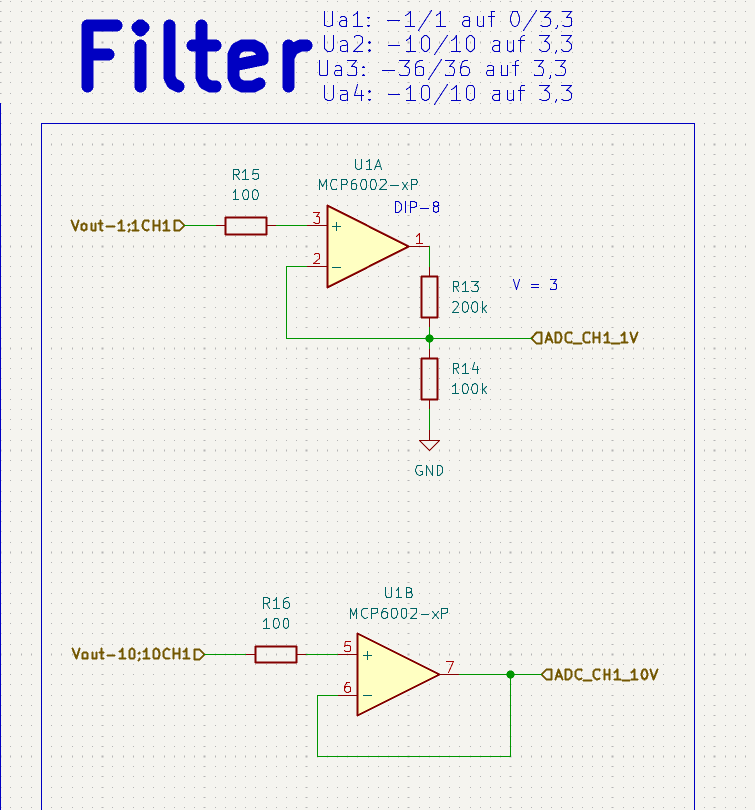
\includegraphics[width=0.7\linewidth]{Filter.png}
		\caption{Nichtinvertierender Verstärker und Impedanzwandler (CH1)}
	\end{figure}
	
	Der obere OPV arbeitet als nichtinvertierender Verstärker (für den \(\pm1\,\mathrm{V}\)-Bereich).
	Die Verstärkung ergibt sich zu
	\[
	V = 1 + \frac{R_{13}}{R_{14}} \approx 3.
	\]
	
	Der Eingangswiderstand \(R_{15}\) dient als HF-Schutz und bildet mit der Eingangskapazität einen kleinen Tiefpass.  
	Der untere OPV ist ein Puffer (Gain = 1) für den \(\pm10\,\mathrm{V}\)-Bereich.
	
	\subsubsection{Schaltungsübersicht und Bauteile CH1}
	
	\begin{figure}[H]
		\centering
		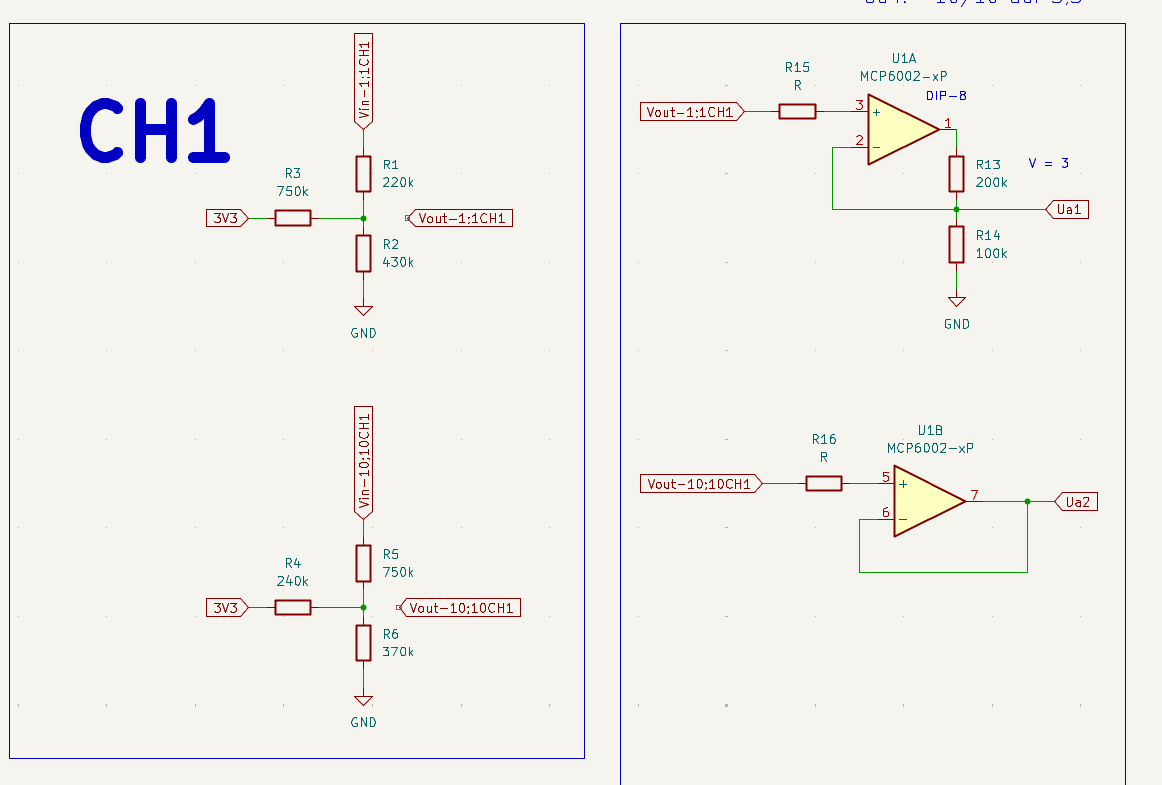
\includegraphics[width=0.95\linewidth]{CH1_messaufbau.png}
		\caption{Schaltung CH1 – Messbereiche \(\pm1\,\mathrm{V}\) und \(\pm10\,\mathrm{V}\)}
	\end{figure}
	
	\begin{table}[H]
		\centering
		\caption{Widerstandswerte CH1 (praktische Umsetzung)}
		\begin{tabular}{lcccc}
			\toprule
			Messbereich & \(R_1\) [k\Omega] & \(R_2\) [k\Omega] & \(R_3\) [k\Omega] & OPV \\
			\midrule
			\(\pm1\,\text{V}\)  & 220 & 430 & 750 & MCP6002 (U1A, \(V = 3\)) \\
			\(\pm10\,\text{V}\) & 750 & 370 & 240 & MCP6002 (U1B) \\
			\bottomrule
		\end{tabular}
	\end{table}
	
	\begin{table}[H]
		\centering
		\renewcommand{\arraystretch}{1.2}
		\caption{Bauteileübersicht für CH1}
		\begin{tabular}{p{2.5cm} p{3.5cm} p{4cm} p{3cm}}
			\toprule
			\textbf{Bezeichnung} & \textbf{Wert} & \textbf{Funktion} & \textbf{Hinweis} \\
			\midrule
			R1, R2, R3 & 220/430/750 k\(\Omega\)
			& Spannungsteiler \(\pm1\,\mathrm{V}\) & Offsetnetzwerk \\[2pt]
			R4, R5, R6 & 240/750/370 k\(\Omega\)
			& Spannungsteiler \(\pm10\,\mathrm{V}\) & Offsetnetzwerk \\[2pt]
			R13, R14   & 200/100 k\(\Omega\)
			& Nichtinvertierender Verstärker (\(V=3\)) & Bereich \(\pm1\,\mathrm{V}\) \\[2pt]
			R15, R16   & 100 \(\Omega\)–1 k\(\Omega\)
			& Serienwiderstände & Eingangsschutz \\[2pt]
			U1A, U1B   & MCP6002 & Buffer / Verstärker & Rail-to-Rail OPV \\
			\bottomrule
		\end{tabular}
	\end{table}
	
	\paragraph{Fazit CH1}
	
	Die Schaltung CH1 funktioniert wie geplant.  
	Der nichtinvertierende Verstärker im \(\pm1\,\mathrm{V}\)-Bereich skaliert das Ausgangssignal auf \(0\dots 3{,}3\,\mathrm{V}\).  
	Die \(\pm10\,\mathrm{V}\)-Stufe liefert stabile Ergebnisse.  
	Durch den MCP6002 als Buffer bleibt die Eingangsimpedanz hoch und der ADC wird gut angesteuert.
	
	% ---------------------------------------------------------
	\subsection{Analoges Frontend – Channel 2 (CH2)}
	
	\begin{figure}[H]
		\centering
		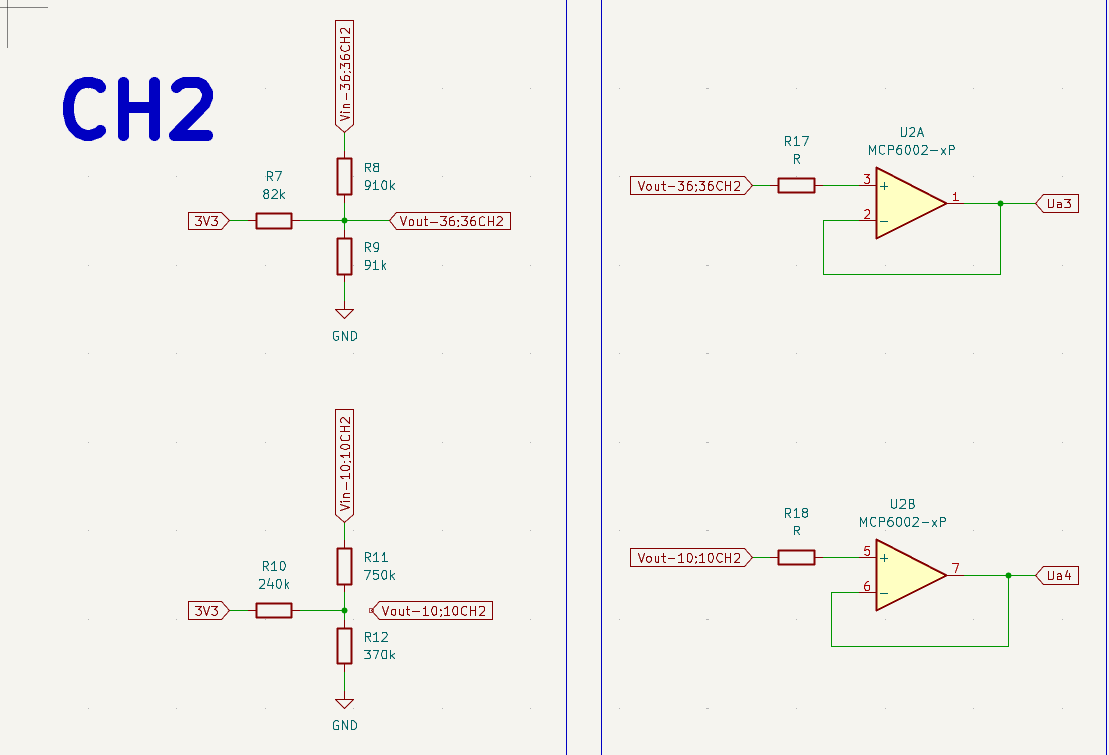
\includegraphics[width=0.95\linewidth]{CH2_messaufbau.png}
		\caption{Schaltung CH2 – Messbereiche \(\pm10\,\mathrm{V}\) und \(\pm36\,\mathrm{V}\)}
	\end{figure}
	
	\begin{table}[H]
		\centering
		\caption{Widerstandswerte CH2 (praktische Umsetzung)}
		\begin{tabular}{lcccc}
			\toprule
			Messbereich & \(R_1\) [k\Omega] & \(R_2\) [k\Omega] & \(R_3\) [k\Omega] & OPV \\
			\midrule
			\(\pm36\,\text{V}\) & 910 & 91  & 82  & MCP6002 (U2A) \\
			\(\pm10\,\text{V}\) & 750 & 370 & 240 & MCP6002 (U2B) \\
			\bottomrule
		\end{tabular}
	\end{table}
	
	\begin{table}[H]
		\centering
		\caption{Bauteile für CH2}
		\begin{tabular}{llll}
			\toprule
			Bezeichnung & Wert & Funktion & Hinweis \\
			\midrule
			R7, R8, R9    & 82/910/91 k\(\Omega\) & Spannungsteiler \(\pm36\,\mathrm{V}\) & Offsetnetzwerk \\
			R10, R11, R12 & 240/750/370 k\(\Omega\) & Spannungsteiler \(\pm10\,\mathrm{V}\) & Offsetnetzwerk \\
			R17, R18      & 100 \(\Omega\)–1 k\(\Omega\) & Serienwiderstände & Eingangsbegrenzung \\
			U2A, U2B      & MCP6002 & Impedanzwandler & Rail-to-Rail OPV \\
			\bottomrule
		\end{tabular}
	\end{table}
	
	\subsubsection{Messaufbau CH2}
	
%	\begin{figure}[H]
%		\centering
%		\includegraphics[width=0.7\linewidth]{CH2messaufbau.png}
%		\caption{Messaufbau für CH2 – Versorgung, Signalgenerator und Multimeter}
%	\end{figure}
	
	Zur Verifikation wurden Messungen mit \(\pm10\,\mathrm{V}\) und \(\pm36\,\mathrm{V}\) (Sinus und DC) durchgeführt.  
	Die Offsetversorgung \(U_\text{ref} = 3{,}3\,\mathrm{V}\) wurde vom gleichen Regler wie der µC gespeist.  
	Gemessen wurde jeweils hinter dem Impedanzwandler.
	
	Ergebnis:
	\[
	U_\text{out,max} \approx 3{,}28\,\mathrm{V}, \quad U_\text{out,min} \approx 0{,}04\,\mathrm{V}.
	\]
	
	\paragraph{Fazit CH2}
	
	Beide Spannungsteiler und Buffer funktionieren wie berechnet.  
	Der parallele Betrieb beider Messbereiche ist stabil, da die OPV-Stufen voneinander entkoppelt sind.  
	Die gemessenen Spannungen liegen innerhalb der Toleranz.
	
	% ---------------------------------------------------------
	\subsection{Wahl der ADC-Pins}
	
	Für die ADC-Signale wurden Pins aus Port A (PA0–PA7) verwendet, die direkt mit ADC1 des STM32L432KC verbunden sind.  
	Dadurch entstehen keine Konflikte mit anderen Peripherien (UART, SPI, I\textsuperscript{2}C), und alle Messkanäle liegen am gleichen ADC-Block.
	
	% ---------------------------------------------------------
	\subsection*{Eingangsstromberechnung und Schutzbetrachtung}
	
	Um den Aufbau zu vereinfachen, wird zwischen den Messbereichen nicht per Relais umgeschaltet.  
	Alle Bereiche liegen parallel über eigene Spannungsteiler am ADC.
	
	Für den größten Bereich (\(\pm 36\,\mathrm{V}\)) gilt mit den praktischen Werten
	\(R_1 = \SI{910}{k\ohm}\), \(R_2 = \SI{91}{k\ohm}\):
	
	\[
	I_{\text{in,max}} = \frac{36\,\mathrm{V} - 3.3\,\mathrm{V}}{R_1 + R_2}
	= \frac{32{,}7\,\mathrm{V}}{1{,}001\,\mathrm{M\Omega}}
	\approx 33\,\mu\mathrm{A}.
	\]
	
	Laut Datenblatt des MCP6002 sind Eingangsschutzströme bis \(\pm 2\,\mathrm{mA}\) zulässig.  
	Der berechnete Strom liegt mehr als Faktor 50 darunter.  
	Eine zusätzliche Schutzbeschaltung (z.\,B. Seriendioden) ist daher nicht nötig.
	
	% ---------------------------------------------------------
	\subsection{Tastkopfabgleich}
	
	In der Eingangsschaltung wurde ein kleiner Kondensator (\(C_1 = \SI{12}{pF}\)) parallel zu \(R_3\) eingebaut, um den Tastkopfabgleich zu ermöglichen.
	Dieser Kondensator gleicht die Kapazität des Tastkopfs aus und sorgt dafür, dass der Spannungsteiler bei hohen Frequenzen genauso teilt wie bei tiefen Frequenzen.
	Ohne diesen Abgleich würden schnelle Flanken verzerrt oder abgerundet.  
	Mit dem Kondensator bleibt die Signalform stabil; das gleiche Prinzip wird auch in professionellen Oszilloskopen verwendet.
	
	% ---------------------------------------------------------
	\subsection{Versorgungsspannung und Spannungsregler}
	
	\begin{figure}[H]
		\centering
		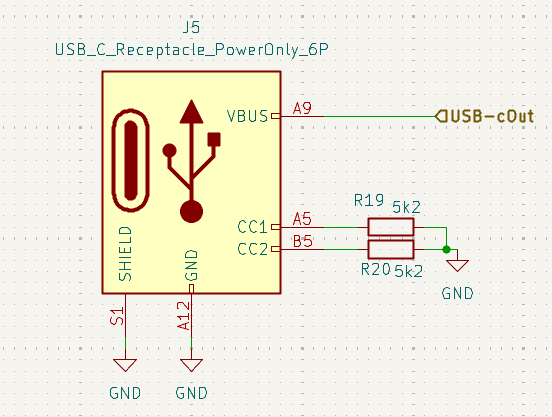
\includegraphics[width=0.7\linewidth]{Receptacle.png}
		\caption{USB-C-Port (J5)}
	\end{figure}
	
	Der USB-C-Port liefert \SI{5}{V} am VBUS-Pin.  
	Die CC1- und CC2-Pins sind mit je einem \SI{5.2}{k\ohm}-Widerstand gegen Masse beschaltet, sodass sich das Board als „Sink“ anmeldet.
	
	\begin{figure}[H]
		\centering
		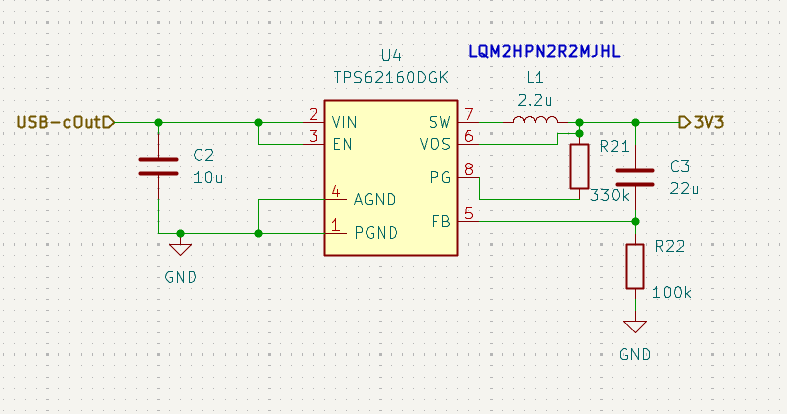
\includegraphics[width=0.9\linewidth]{PowerSupply2.png}
		\caption{TPS62160-Schaltregler}
	\end{figure}
	
	Für die Spannungsversorgung wird ein \textbf{TPS62160DGKR} eingesetzt.  
	Er wandelt die \SI{5}{V} des USB-C-Anschlusses in eine stabile \SI{3.3}{V}-Schiene um.  
	Der auf dem NUCLEO-L432KC vorhandene Linearregler wäre thermisch schnell am Limit, da das System (MCU, Ethernet, Display) bis zu ca. \SI{300}{mA} ziehen kann.  
	Der Schaltregler arbeitet mit hohem Wirkungsgrad und bleibt deutlich kühler.
	
	Die Ausgangsspannung wird über einen Widerstandsteiler am Feedback-Pin eingestellt:
	\[
	V_\text{OUT} = 0{,}8\,\mathrm{V} \left(1 + \frac{R_{21}}{R_{22}}\right).
	\]
	
	Mit \(R_{21} = \SI{330}{k\ohm}\) und \(R_{22} = \SI{100}{k\ohm}\) ergibt sich etwa \(V_\text{OUT} \approx \SI{3.4}{V}\), was innerhalb der Toleranzen aller \SI{3.3}{V}-Bauteile liegt.
	
	Zur Glättung dienen:
	\begin{itemize}
		\item Eingangskondensator $C_2$,
		\item Induktivität $L_1$,
		\item Ausgangskondensator $C_3$.
	\end{itemize}
	
	Diese Werte entsprechen der Referenzschaltung von Texas Instruments.
	
	% ---------------------------------------------------------
	\subsection{Display-Anschluss}
	
	\begin{figure}[H]
		\centering
		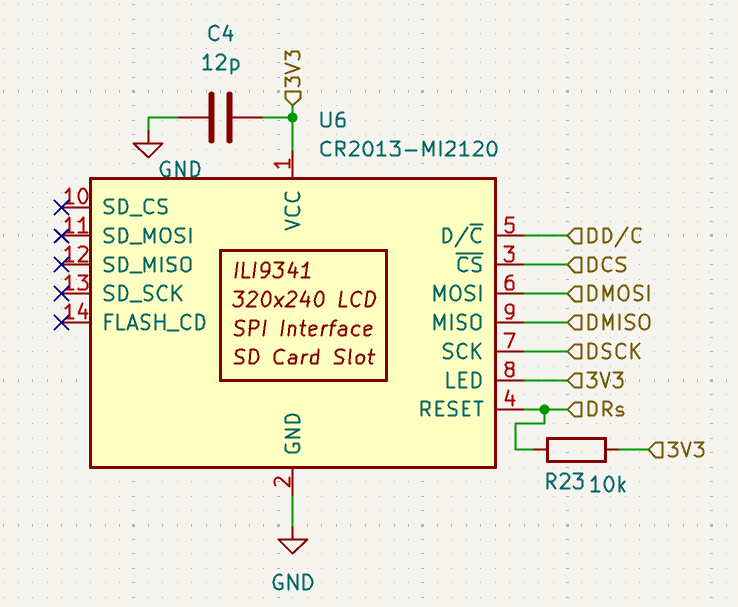
\includegraphics[width=0.7\linewidth]{Display.png}
		\caption{ILI9341-Display-Anschluss}
	\end{figure}
	
	Das ILI9341-Modul wird mit \SI{3.3}{V} versorgt.  
	Ein Kondensator direkt am Modul stabilisiert die Versorgung.  
	Die Datenübertragung erfolgt über SPI (MOSI, MISO, SCK, CS, D/C).  
	RESET wird über einen \SI{10}{k\ohm}-Pull-up auf \SI{3.3}{V} gehalten.
	
	% =========================================================
	\section{Layout-Grundlagen (kurz)}
	
	Beim Layout wurden folgende Punkte beachtet:
	\begin{itemize}
		\item Getrennte Bereiche für Analog- und Digitalsignale, um Störungen zu verringern.
		\item Durchgehende Massefläche (GND-Plane) auf einer Lage.
		\item Kurze Leitungen für die analogen Signale zwischen Spannungsteiler, OPV und ADC.
		\item ESD-Schutz und saubere Führung der Koax-Masse direkt zum Eingang.
		\item Abblockkondensatoren nahe an den Versorgungspins von OPV und µC.
	\end{itemize}
	
	\begin{figure}[H]
		\centering
		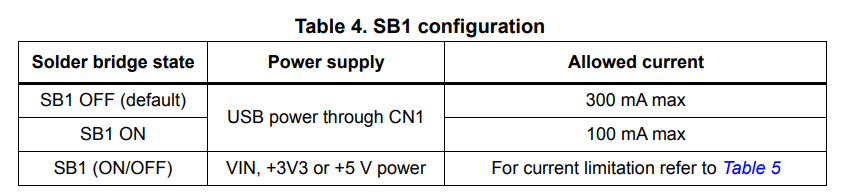
\includegraphics[width=0.5\linewidth]{On-board-spgregler.png}
		\caption{Ausschnitt: Onboard-Spannungsregler im Layout}
	\end{figure}
	
	% =========================================================

	\section*{Abkürzungen}
	
	\begin{description}
		\item[Oszi]   Oszilloskop
		\item[KS]     Kurzschluss
		\item[LL]     Leerlauf
		\item[\(R_2 \parallel R_3\)]  Parallelschaltung zweier Widerstände
		\item[ADC]    Analog-Digital-Umsetzer (Analog-to-Digital Converter)
	\end{description}
	
	\section*{Quelle}
	
	\noindent
	Datenblätter MCP6002, TPS62160, STM32L432KC, ILI9341, W5500.  
	Eigene Simulationen und Messungen im Labor.
	
	
	\begin{tikzpicture}
		\begin{axis}[
			xlabel={Zeit (s)},
			ylabel={Spannung (V)},
			grid=both
			]
			\addplot[
			blue,
			very thick
			]
			table[
			col sep=comma
			] {CLK.csv};
		\end{axis}
	\end{tikzpicture}
	
\end{document}
